% ECE 579 — Solar PV Machine Learning Project
% Standalone Beamer presentation. Compile this file (ppt.tex) in the SAME
% Overleaf project as main.tex; it reuses Assets/ and Figures/ without copying.
%
% SPEAKER NOTES: every slide carries a short narration script in \note{...}.
%   * Default (below): notes hidden -> normal slide deck for the video.
%   * To print the script, uncomment ONE of the lines marked "NOTES" below:
%       \setbeameroption{show only notes}            -> notes pages only (script)
%       \setbeameroption{show notes on second screen=right}  -> slide + notes side by side
%     (the second-screen option needs \usepackage{pgfpages}, already loaded).
\documentclass[aspectratio=169,11pt]{beamer}
\usepackage[T1]{fontenc}
\usepackage{lmodern}
\usepackage{graphicx}
\usepackage{booktabs}
\usepackage{array}
\usepackage{tabularx}
\usepackage{tikz}
\usetikzlibrary{arrows.meta,positioning,calc,shapes.geometric}
\usepackage[table]{xcolor}
\usepackage{amsmath}
\usepackage{adjustbox}
\usepackage{pgfpages}
% NOTES: \setbeameroption{show only notes}
% NOTES: \setbeameroption{show notes on second screen=right}

% -------------------------------------------------------------
% STANDARD ACADEMIC BEAMER STYLE
% -------------------------------------------------------------
\usetheme{Madrid}
\usecolortheme{default}
\usefonttheme{professionalfonts}
\setbeamertemplate{navigation symbols}{}
\setbeamertemplate{blocks}[default]
\setbeamertemplate{items}[default]
\setbeamersize{text margin left=0.65cm,text margin right=0.65cm}
\setbeamerfont{note page}{size=\small}

\definecolor{navy}{HTML}{25456A}
\definecolor{teal}{HTML}{32658E}
\definecolor{gold}{HTML}{6F8495}
\definecolor{softblue}{HTML}{F2F6FB}
\definecolor{softteal}{HTML}{EAF1F7}
\definecolor{softgold}{HTML}{F4F6F8}
\definecolor{ink}{HTML}{263441}
\definecolor{slate}{HTML}{667581}
\definecolor{lightborder}{HTML}{B8C7D5}
\definecolor{warn}{HTML}{B5562B}

\title[PV Power Prediction]{Solar Photovoltaic Power Prediction}
\subtitle{A Multi-Paradigm Machine Learning Study}
\author[Albert Shaju]{Albert Shaju}
\institute[WPI]{Worcester Polytechnic Institute\\[2pt]
ECE 579: Machine Learning for Engineering Applications\\
Instructor: Prof. Ziming Zhang}
\date[Nov. 2026]{November 2026}
\titlegraphic{
\includegraphics[height=1.2cm,keepaspectratio]{Assets/WPI_seal_from_uploaded_logo.png}}

\newcommand{\sectiontag}[1]{{\footnotesize\usebeamercolor[fg]{structure}\textbf{#1}}\par\vspace{0.10cm}}
\newcommand{\smallmuted}[1]{{\footnotesize\color{slate}#1\par}}
\newcommand{\factbox}[2]{\begin{beamercolorbox}[sep=0.13cm,wd=\linewidth]{block body}{\bfseries #1}\par\small #2\end{beamercolorbox}}
\newcommand{\footeridea}[1]{\par\vspace{0.08cm}{\footnotesize\textbf{Key point:} #1}}
\newcolumntype{Y}{>{\raggedright\arraybackslash}X}
\newcolumntype{P}[1]{>{\raggedright\arraybackslash}p{#1}}


% Change to \showbackuptrue to generate detailed backup tables and figures after the main talk.
% Links shown on the title and closing slides.
\newcommand{\videourl}{https://drive.google.com/file/d/1yEQ6FFIMTAmYXIgzWIxX5eqDjJoTPSaY/view?usp=sharing}
\newcommand{\repourl}{https://github.com/myProjects400/ECE579-PV-ML-Project}

\newif\ifshowbackup
\showbackupfalse

\begin{document}
\begin{frame}[plain]
\titlepage
\vspace{-0.35cm}
\begin{center}\scriptsize
\textbf{Video:} \href{\videourl}{\nolinkurl{\videourl}}\\[1pt]
\textbf{Code:} \href{\repourl}{\nolinkurl{\repourl}}
\end{center}
\note{Hi, I'm Albert Shaju. This video walks through my ECE 579 course project on predicting
solar photovoltaic power with machine learning. I'll cover five learning problems built on the
same five-city dataset, explain the methods, show the key results, and finish with the single
most interesting finding.}
\end{frame}


\section{Introduction and Data}

\begin{frame}{Why predict PV output?}
\sectiontag{MOTIVATION}
\begin{columns}[T,totalwidth=\textwidth]
\begin{column}{0.50\textwidth}
\begin{block}{The grid problem}
\small
\begin{itemize}\setlength\itemsep{0.30em}
\item PV is one of the fastest-growing electricity sources.
\item Output follows the weather: irradiance, clouds and temperature change minute to minute.
\item Operators need \textbf{very-short-term} estimates to balance load, smooth ramps and schedule storage.
\end{itemize}
\end{block}
\end{column}
\begin{column}{0.46\textwidth}
\begin{block}{What makes it hard here}
\small
\begin{itemize}\setlength\itemsep{0.30em}
\item \textbf{Different scale per city:} max output $\approx$72\,kW (La Jolla) to $\approx$263\,kW (Davis).
\item \textbf{Time series:} no random shuffling.
\item \textbf{Scarce labels:} sensors fail; new sites have little history.
\item \textbf{New sites:} models must travel between cities.
\end{itemize}
\end{block}
\end{column}
\end{columns}
\footeridea{Each of these difficulties becomes one of the five project problems.}
\note{Why does this matter? Solar output is intermittent: it follows irradiance, clouds and
temperature. Grid operators need short-horizon estimates to balance load and plan storage.
Four things make this dataset hard: each city has a very different power scale, the data is a
time series, labels can be scarce, and we often need a model in a city where we have little data.}
\end{frame}





\begin{frame}{Dataset and experimental design}
\sectiontag{DATA AND PROTOCOL}
\begin{columns}[T,totalwidth=\textwidth]
\begin{column}{0.53\textwidth}
\begin{block}{Measurements}
\small
\begin{itemize}
\setlength\itemsep{0.15em}
\item \textbf{Nine city sheets}, 30-min samples, 10:00--14:30 solar time.
\item Davis, Huron, Santa Barbara, La Jolla: 2011--2016 and 2014--2016.
\item Amherst: 2018--2020 only.
\item 22 columns: DHI/DNI/GHI, clear-sky values, Cloud Type, temperature, humidity, wind, pressure, zenith angle, \textbf{Output Power}.
\end{itemize}
\end{block}
\end{column}
\begin{column}{0.44\textwidth}
\begin{block}{Consistent evaluation}
\small
\begin{itemize}
\setlength\itemsep{0.25em}
\item \textbf{Chronological 80/20 split}: earlier for training, later for testing.
\item \textbf{Seeds:} 42, 123, 2026; mean $\pm$ SD.
\item \textbf{Metrics:} balanced accuracy, macro-F1; RMSE, MAE, nRMSE.
\end{itemize}
\end{block}
\end{column}
\end{columns}
\vspace{-0.15cm}
\[
\mathrm{nRMSE}(\%) = 100\cdot\frac{\mathrm{RMSE}}{\max(y_{\mathrm{test}})-\min(y_{\mathrm{test}})}
\quad\text{makes errors comparable across cities.}
\]
\note{The workbook has nine sheets: four cities with three- and six-year versions, plus Amherst
with three years. Each row is a 30-minute measurement around midday. Every experiment uses a
chronological 80/20 split and three seeds. Because each city has a different power scale, I
report normalized RMSE, which divides the error by the test-set power range.}
\end{frame}


\begin{frame}{Leakage-safe preprocessing: fit on training observations}
\sectiontag{SHARED PIPELINE}
\centering
\begin{adjustbox}{max width=\linewidth,max totalheight=4.90cm}
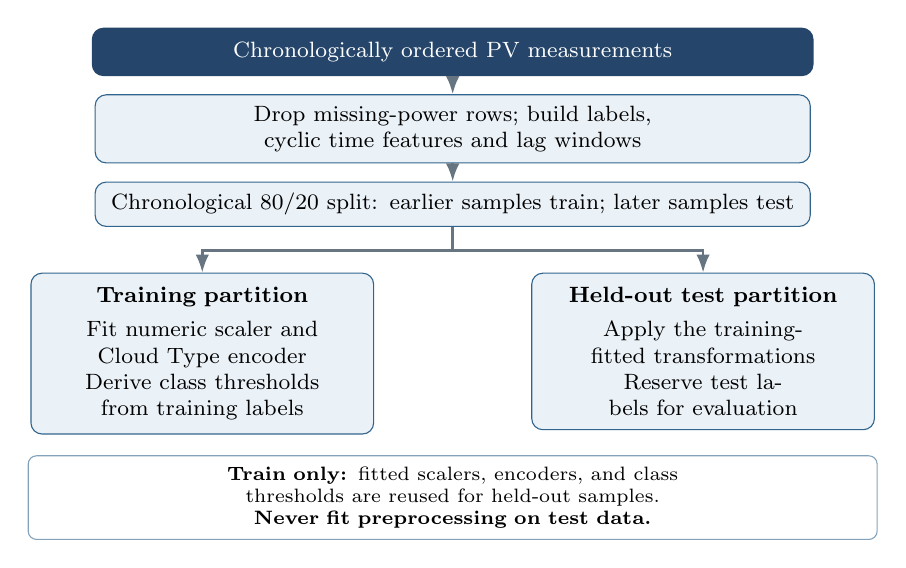
\begin{tikzpicture}[>=Latex,node distance=0.26cm,
  every node/.style={align=center},
  data/.style={draw=navy,fill=navy,text=white,rounded corners=4pt,
               text width=8.8cm,minimum height=0.55cm,font=\footnotesize,inner sep=5pt},
  stepbox/.style={draw=teal,fill=softteal,rounded corners=4pt,
               text width=8.8cm,minimum height=0.52cm,font=\footnotesize,inner sep=4pt},
  branchbox/.style={draw=teal,fill=softteal,rounded corners=4pt,
                 text width=4.0cm,minimum height=1.14cm,
                 inner sep=5pt,font=\footnotesize},
  arrow/.style={-{Latex[length=2.3mm]},draw=slate,line width=0.95pt},
  connector/.style={draw=slate,line width=0.95pt}]
  \node[data] (raw) {Chronologically ordered PV measurements};
  \node[stepbox,below=0.23cm of raw] (prepare)
      {Drop missing-power rows; build labels, cyclic time features and lag windows};
  \node[stepbox,below=0.23cm of prepare] (split)
      {Chronological 80/20 split: earlier samples train; later samples test};
  \node[branchbox,below=0.58cm of split,xshift=-3.18cm] (train)
     {\textbf{Training partition}\\[3pt]
      Fit numeric scaler and Cloud Type encoder\\
      Derive class thresholds from training labels};
  \node[branchbox,below=0.58cm of split,xshift=3.18cm] (test)
     {\textbf{Held-out test partition}\\[3pt]
      Apply the training-fitted transformations\\
      Reserve test labels for evaluation};
  \draw[arrow] (raw.south) -- (prepare.north);
  \draw[arrow] (prepare.south) -- (split.north);
  \coordinate (fork) at ($(split.south)+(0,-0.30cm)$);
  \draw[connector] (split.south) -- (fork);
  \draw[arrow] (fork) -| (train.north);
  \draw[arrow] (fork) -| (test.north);
  \coordinate (under) at ($(train.south)!0.5!(test.south)$);
  \node[draw=teal!60,fill=white,rounded corners=3pt,text width=10.50cm,
        font=\scriptsize,inner sep=4pt,below=0.29cm of under] (note)
    {\textbf{Train only:} fitted scalers, encoders, and class thresholds are reused for held-out samples.\\
     \textbf{Never fit preprocessing on test data.}};
\end{tikzpicture}
\end{adjustbox}
\note{This pipeline is shared by every problem. I sort by time, split first, and only then fit
anything. The scaler, the Cloud Type one-hot encoder and the class thresholds are learned from the
training partition and simply applied to the test partition. That way no information from the
future leaks into training.}
\end{frame}




\section{P1: Supervised Classification}

\begin{frame}{Problem 1 — Supervised Classification}
\sectiontag{P1 \quad PROBLEM}
\begin{block}{Objective from the assignment}
Predict a \textbf{discrete label} from meteorological and irradiance features.
\end{block}
\vspace{0.02cm}
\begin{columns}[T,totalwidth=\textwidth]
\begin{column}{0.49\textwidth}
\begin{block}{Task A: Sky-condition class}
\small Three classes using $k=\mathrm{GHI}/\mathrm{Clearsky\ GHI}$:\\[2pt]
Clear ($k\ge0.85$), Partly Cloudy ($0.4\le k<0.85$), Overcast ($k<0.4$).
\end{block}
\end{column}
\begin{column}{0.49\textwidth}
\begin{block}{Task B: Generation-regime class}
\small Bin Output Power into city-specific terciles:\\[3pt]
\textbf{Low / Medium / High}.
\end{block}
\end{column}
\end{columns}
\vspace{0.10cm}
\begin{block}{Deliverable in the question}
\small Classification pipeline, confusion matrix and per-class metrics; identify which classes are hardest and why.
\end{block}
\note{Problem 1 has two classification tasks. The sky task uses the clear-sky index, GHI divided
by clear-sky GHI, to define Clear, Partly Cloudy and Overcast. The generation task splits output
power into Low, Medium and High terciles for each city. The question also asks which classes are
hardest and why, and I'll answer that directly.}
\end{frame}

\begin{frame}{P1 — Preprocessing and labels}
\sectiontag{P1 \quad PREPROCESSING}
\begin{enumerate}\setlength\itemsep{0.40em}
\item \textbf{Chronological separation:} earlier 80\% for training, last 20\% for testing.
\item \textbf{Sky target:} $k=\mathrm{GHI}/\mathrm{Clearsky\ GHI}$; Overcast if $k<0.4$, Partly Cloudy if $0.4\le k<0.85$, Clear otherwise.
\item \textbf{Generation target:} Low/Medium/High from \textbf{training-set} terciles, applied unchanged to test.
\item \textbf{No label leakage:} remove GHI and Clearsky GHI for Sky (and test a variant without Output Power); remove Output Power for Generation.
\item \textbf{Train-fitted transformation:} scaling and one-hot Cloud Type.
\end{enumerate}
\footeridea{The test set never determines scaling parameters or class boundaries.}
\note{To avoid leakage, the columns that define a label are removed from its inputs. For the sky
task I drop GHI and clear-sky GHI, and I also run a variant without Output Power to check it is
not a shortcut. For the generation task I drop Output Power. Tercile thresholds come from the
training data only.}
\end{frame}

\begin{frame}{P1 — Models: classical ML and deep learning}
\sectiontag{P1 \quad MODELS}
\renewcommand{\arraystretch}{1.32}
\begin{tabularx}{\linewidth}{@{}P{2.25cm}YYP{2.4cm}@{}}\toprule
\textbf{Family} & \textbf{Models evaluated} & \textbf{Purpose} & \textbf{Library}\\\midrule
\rowcolor{softblue} Classical ML & Logistic regression, RBF SVM & Linear and kernel boundaries & scikit-learn\\
\rowcolor{softblue} Classical ML & Random forest, XGBoost & Bagged and boosted trees & scikit-learn, xgboost\\
\rowcolor{softteal} Deep learning & MLP & Nonlinear neural classifier & PyTorch\\\bottomrule
\end{tabularx}\par
\vspace{0.13cm}
\begin{block}{Evaluation protocol}
\small Five classifiers $\times$ two tasks $\times$ two cities; balanced accuracy and macro-F1 as mean $\pm$ SD over three seeds.
\end{block}
\footeridea{Linear, kernel, tree-based, boosting and neural families are all represented.}
\note{I compare five classifiers that cover the main model families: logistic regression,
an RBF-kernel SVM, random forest, XGBoost, and a PyTorch multilayer perceptron. Every number is a
mean over three seeds.}
\end{frame}

\begin{frame}{P1 — All classifiers: Davis test results}
\sectiontag{P1 \quad RESULTS — DAVIS}
\smallmuted{Five fixed classifier families, each trained separately for Sky and Generation. Held-out BA/Macro-F1 (mean $\pm$ SD, \%, 3 seeds); bold = best for that task.}
\vspace{0.14cm}
{\scriptsize
\setlength{\tabcolsep}{5.2pt}
\renewcommand{\arraystretch}{1.55}
\begin{tabular}{@{}lrrrr@{}}\toprule
\textbf{Classifier} & \textbf{Sky BA} & \textbf{Sky Macro-F1} & \textbf{Generation BA} & \textbf{Gen. Macro-F1}\\\midrule
Logistic regression & 98.60 $\pm$ 0.00 & 98.02 $\pm$ 0.00 & 94.90 $\pm$ 0.00 & 94.90 $\pm$ 0.00\\
RBF SVM & 97.51 $\pm$ 0.00 & 96.60 $\pm$ 0.00 & 95.32 $\pm$ 0.00 & 95.35 $\pm$ 0.00\\
Random forest$^{\dagger}$ & 98.65 $\pm$ 0.13 & 98.34 $\pm$ 0.10 & 95.96 $\pm$ 0.08 & 96.05 $\pm$ 0.08\\
\rowcolor{softteal} XGBoost$^{\dagger}$ & \textbf{99.15 $\pm$ 0.15} & \textbf{99.11 $\pm$ 0.11} & \textbf{96.35 $\pm$ 0.09} & \textbf{96.43 $\pm$ 0.09}\\
MLP (PyTorch) & 98.19 $\pm$ 0.18 & 97.76 $\pm$ 0.47 & 94.98 $\pm$ 0.43 & 94.99 $\pm$ 0.43\\
\bottomrule\end{tabular}
}
\vspace{0.18cm}
\begin{block}{Interpretation}
\small XGBoost is best on both Davis tasks. Logistic regression is within 0.6 points on Sky, so the sky task is nearly linearly separable. $\dagger$ = validation-selected model.
\end{block}
\note{Here are all five classifiers for Davis. XGBoost wins both tasks. Notice that plain logistic
regression is only about half a point behind on the sky task, which tells us the sky classes are
almost linearly separable from the remaining correlated meteorological and irradiance measurements. Deterministic models show a
standard deviation of zero.}
\end{frame}

\begin{frame}{P1 — All classifiers: Amherst test results}
\sectiontag{P1 \quad RESULTS — AMHERST}
\smallmuted{Five fixed classifier families, each trained separately for Sky and Generation. Held-out BA/Macro-F1 (mean $\pm$ SD, \%, 3 seeds); bold = best for that task.}
\vspace{0.14cm}
{\scriptsize
\setlength{\tabcolsep}{5.2pt}
\renewcommand{\arraystretch}{1.55}
\begin{tabular}{@{}lrrrr@{}}\toprule
\textbf{Classifier} & \textbf{Sky BA} & \textbf{Sky Macro-F1} & \textbf{Generation BA} & \textbf{Gen. Macro-F1}\\\midrule
Logistic regression & 98.55 $\pm$ 0.00 & 98.48 $\pm$ 0.00 & 73.91 $\pm$ 0.00 & 73.98 $\pm$ 0.00\\
RBF SVM & 97.66 $\pm$ 0.00 & 97.54 $\pm$ 0.00 & 75.27 $\pm$ 0.00 & 75.40 $\pm$ 0.00\\
Random forest & 98.43 $\pm$ 0.02 & 98.19 $\pm$ 0.02 & \cellcolor{softteal}\textbf{75.90 $\pm$ 0.31} & \cellcolor{softteal}\textbf{75.77 $\pm$ 0.31}\\
XGBoost$^{\dagger}$ & \cellcolor{softteal}\textbf{98.82 $\pm$ 0.08} & \cellcolor{softteal}\textbf{98.74 $\pm$ 0.08} & 75.41 $\pm$ 0.06 & 75.22 $\pm$ 0.06\\
MLP (PyTorch)$^{\dagger}$ & 98.11 $\pm$ 0.31 & 98.09 $\pm$ 0.23 & 75.00 $\pm$ 0.47 & 74.85 $\pm$ 0.36\\
\bottomrule\end{tabular}
}
\vspace{0.18cm}
\begin{block}{Interpretation}
\small XGBoost leads Sky; random forest leads Generation. All five models land between 73.9\% and 75.9\% on Amherst Generation: the task remains challenging for all evaluated model families.
\end{block}
\note{In Amherst, the sky task is still easy, but on generation every model lands between about 74 and
76 percent. When five very different model families hit the same ceiling, the task appears difficult for each model family tested.}
\end{frame}

\begin{frame}{P1 — Davis sky confusion matrices}
\sectiontag{P1 \quad RESULTS — DAVIS SKY}
\centering
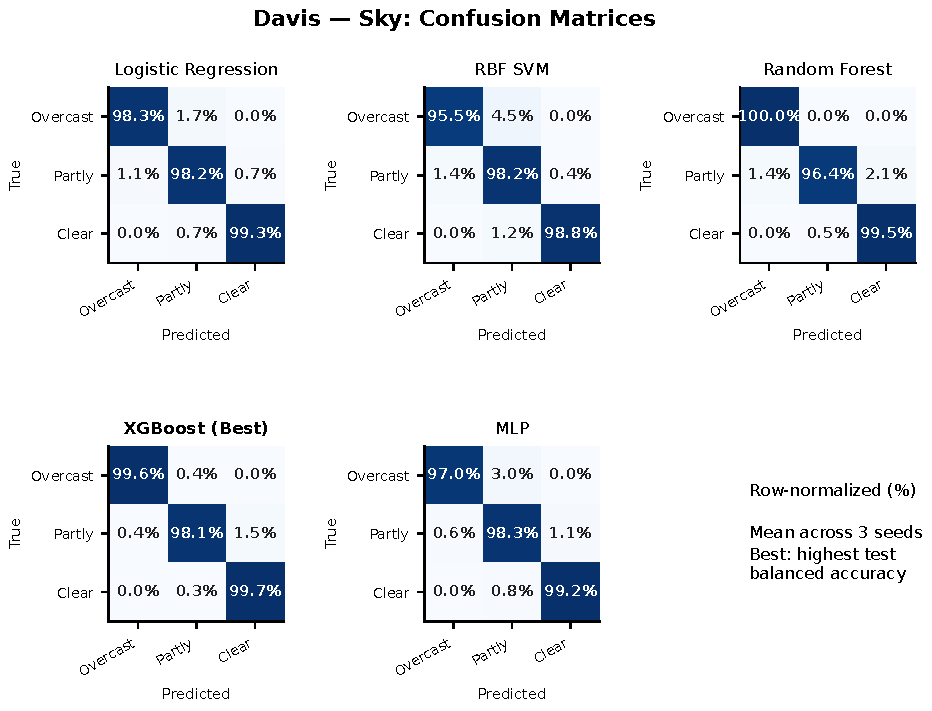
\includegraphics[width=0.93\linewidth,height=5.55cm,keepaspectratio]{Figures/P1/P1_Davis_Sky_Confusion.pdf}\par
\vspace{0.08cm}
\smallmuted{Best model: XGBoost. The few errors involve \textit{Partly Cloudy} and its neighbours.}
\footeridea{Rows are true classes, columns are predicted classes; diagonal values are recall.}
\note{These are the Davis sky confusion matrices for all five models, averaged over seeds. The
diagonal is the recall of each class. The few mistakes are almost all between Partly Cloudy and
one of its neighbours.}
\end{frame}

\begin{frame}{P1 — Amherst sky confusion matrices}
\sectiontag{P1 \quad RESULTS — AMHERST SKY}
\centering
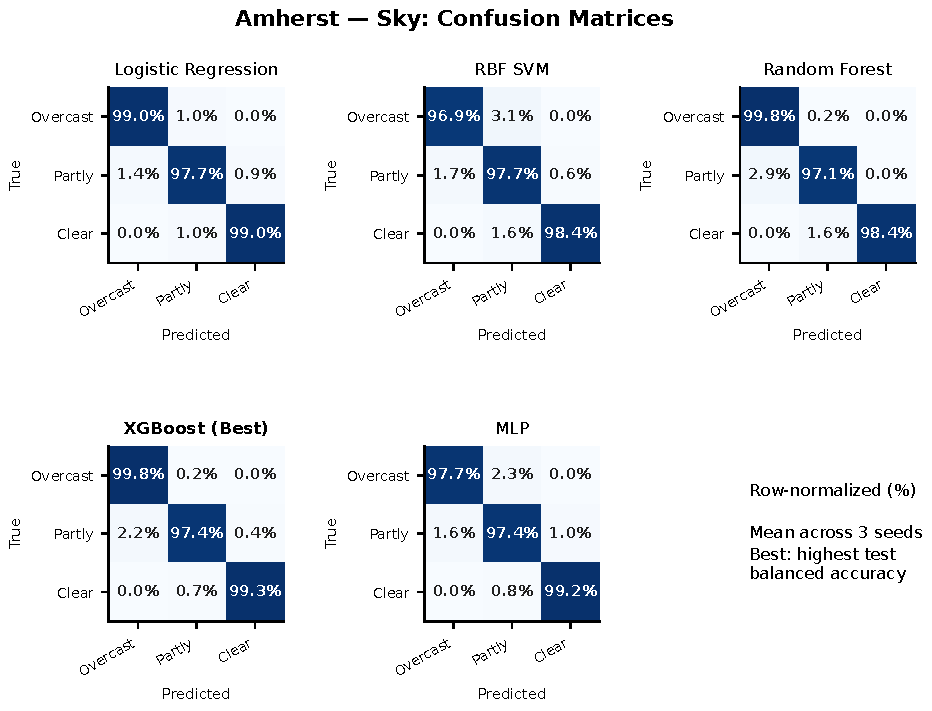
\includegraphics[width=0.93\linewidth,height=5.55cm,keepaspectratio]{Figures/P1/P1_Amherst_Sky_Confusion.pdf}\par
\vspace{0.08cm}
\smallmuted{Best model: XGBoost. \textit{Partly Cloudy} remains hardest because it borders both Overcast and Clear.}
\note{Amherst looks the same: Partly Cloudy is the weakest class, at about 97 percent recall for
the best model.}
\end{frame}

\begin{frame}{P1 — Davis generation confusion matrices}
\sectiontag{P1 \quad RESULTS — DAVIS GENERATION}
\centering
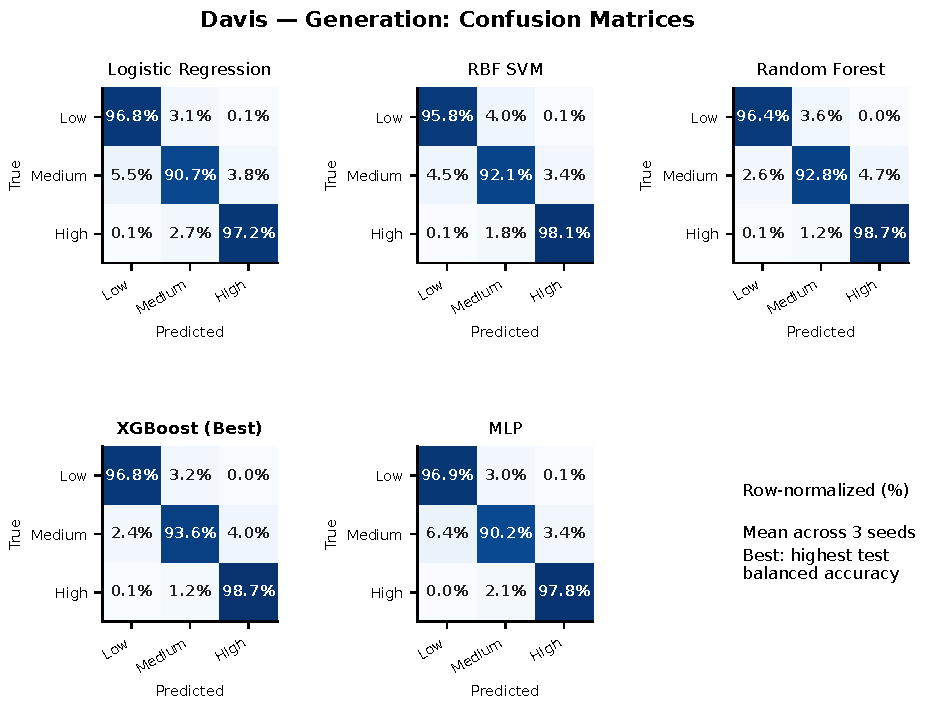
\includegraphics[width=0.93\linewidth,height=5.55cm,keepaspectratio]{Figures/P1/P1_Davis_Generation_Confusion.pdf}\par
\vspace{0.08cm}
\smallmuted{Best model: XGBoost. Most errors are in the \textit{Medium} regime, which lies between Low and High.}
\note{For Davis generation, Medium is the weakest class at about 94 percent recall, still very good.}
\end{frame}

\begin{frame}{P1 — Amherst generation confusion matrices}
\sectiontag{P1 \quad RESULTS — AMHERST GENERATION}
\centering
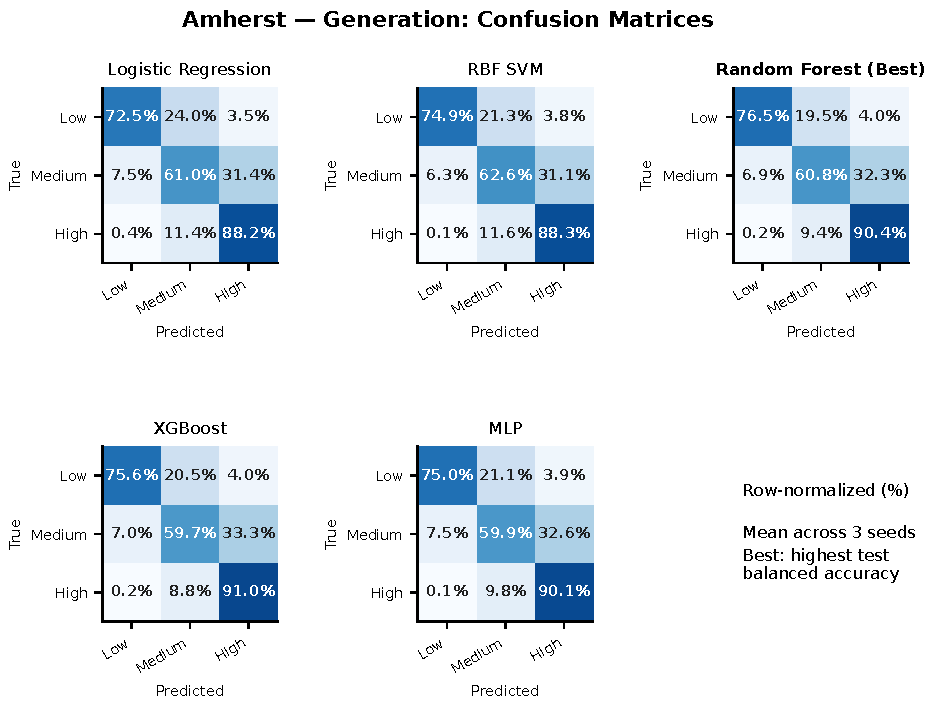
\includegraphics[width=0.93\linewidth,height=5.18cm,keepaspectratio]{Figures/P1/P1_Amherst_Generation_Confusion.pdf}\par
\vspace{0.08cm}
\smallmuted{Best model: random forest. True-\textit{Medium} samples are predicted \textit{High} about 32\% of the time, but \textit{Low} only about 7\%.}
\note{Amherst generation is where things break down. About a third of true Medium samples are
predicted High, but only about seven percent are predicted Low. The error is asymmetric: in Amherst,
weather that looks like a high-output day often produces only medium output.}
\end{frame}

\begin{frame}{P1 — Analysis: why are these classes hardest?}
\sectiontag{P1 \quad ANALYSIS}
\begin{columns}[T,totalwidth=\textwidth]
\begin{column}{0.55\textwidth}
\centering
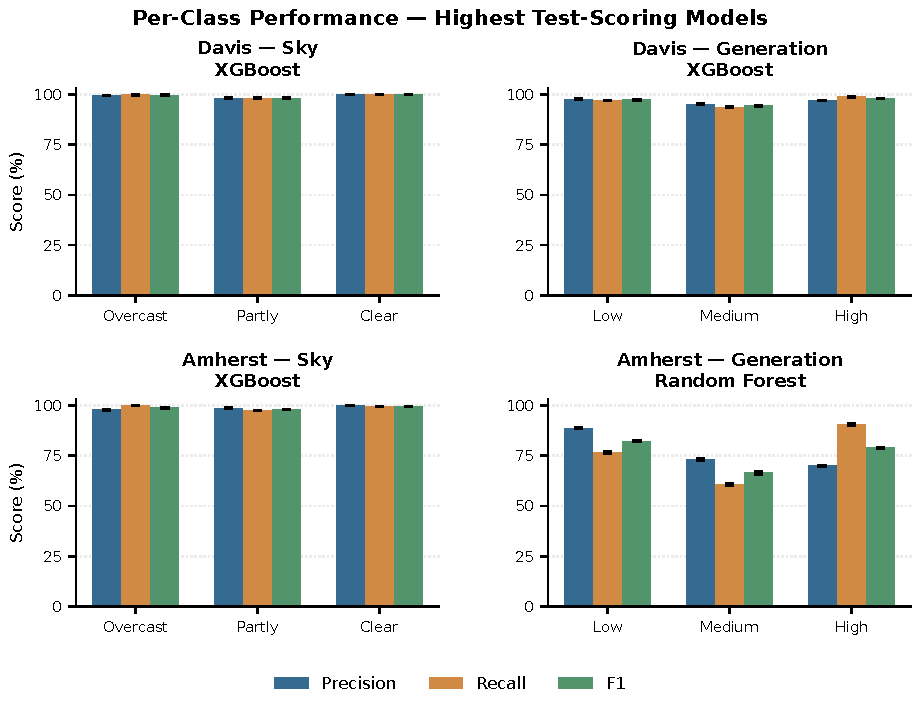
\includegraphics[width=\linewidth,height=5.0cm,keepaspectratio]{Figures/P1/P1_Per_Class_Best_Models.pdf}
\end{column}
\begin{column}{0.42\textwidth}
\factbox{1. Two boundaries}{Middle classes can be wrong in \emph{both} directions; samples near $k{=}0.4$, $k{=}0.85$ or a tercile are ambiguous.}\vspace{0.12cm}
\factbox{2. Weather $\neq$ power in Amherst}{Weather is sensed well (Sky 98.8\%), but the same weather maps to a wider range of output. Snow, soiling, panel temperature or downtime are plausible, unmeasured causes.}
\end{column}
\end{columns}
\footeridea{P2 also shows: Amherst regression error is 15.7\% nRMSE vs 4.7\% in Davis.}
\note{Why? First, middle classes have two decision boundaries, so they can be wrong in either
direction, and samples near a threshold are genuinely ambiguous. Second, in Amherst the weather
itself is classified very well, so the problem is the step from weather to power. Factors like
snow, soiling or downtime are not in the features. The regression results in P2 are consistent with this interpretation.}
\end{frame}



%% Per-problem narrative: objective/methods; all-model results; controlled comparisons; best summary; analysis.
\section{P2: Supervised Regression}

\begin{frame}{Problem 2 — Supervised Regression (Core Task)}
\sectiontag{P2 \quad PROBLEM}
\begin{block}{Objective from the assignment}
Predict continuous \textbf{Output Power (kW)} from the input features.
\end{block}
\vspace{0.01cm}
\begin{columns}[T,totalwidth=\textwidth]
\begin{column}{0.49\textwidth}
\begin{block}{Task A: Same-city}
\small Chronological 80/20 split within Davis and Amherst.
\end{block}
\begin{block}{Task C: Sequential forecasting}
\small Predict the next output from the last $K=12$ steps.
\end{block}
\end{column}
\begin{column}{0.49\textwidth}
\begin{block}{Task B: Cross-city zero-shot}
\small Train on Davis (6 yr); test on Huron, Santa Barbara and La Jolla.
\end{block}
\begin{block}{Task D: History ablation}
\small Three-year versus six-year training history.
\end{block}
\end{column}
\end{columns}
\vspace{0.03cm}
{\small\textbf{Deliverables:} RMSE / MAE / nRMSE for every method and setup; prediction-versus-truth plots.}
\note{Problem 2 is the core regression task, predicting output power in kilowatts. I run four
protocols: same-city, zero-shot cross-city from Davis, a sequential version that uses the last 12
steps to predict the next one, and a three- versus six-year history comparison.}
\end{frame}

\begin{frame}{P2 — Preprocessing and normalization}
\sectiontag{P2 \quad PREPROCESSING}
\begin{enumerate}\setlength\itemsep{0.33em}
\item \textbf{Target:} Output Power is the label; never a contemporaneous input.
\item \textbf{Time split:} chronological 80/20; identical test window for every model.
\item \textbf{Input scaling:} scalers and Cloud Type encoder fitted on the \textbf{training city only}.
\item \textbf{Zero-shot:} reuse \textbf{Davis preprocessing} on target inputs; no target labels, no rescaling of the target output (the strictest setting).
\item \textbf{Sequence:} 12-step history window, including lagged power; no future values.
\end{enumerate}
\vspace{0.03cm}
\smallmuted{nRMSE is an evaluation metric only (RMSE divided by the test power range); it is not an input transformation.}
\note{Preprocessing follows the shared pipeline. One important choice: in the zero-shot
experiment I reuse the Davis preprocessing and do not rescale the output to the target city. That
is the strictest version of zero-shot, and it exposes the scale problem very clearly.}
\end{frame}

\begin{frame}{P2 — Models used}
\sectiontag{P2 \quad MODELS}
\renewcommand{\arraystretch}{1.35}
\begin{tabularx}{\linewidth}{@{}P{2.25cm}YP{3.0cm}@{}}\toprule
\textbf{Family} & \textbf{Evaluated models} & \textbf{Library}\\\midrule
\rowcolor{softblue} Classical ML & Ridge regression, RBF SVR, random forest & scikit-learn\\
\rowcolor{softblue} Classical ML & Gradient-boosted regression trees & XGBoost\\
\rowcolor{softteal} Deep learning & Multilayer perceptron (MLP) & PyTorch\\
\rowcolor{softteal} Deep learning & LSTM over the 12-step window & PyTorch; sequential task\\\bottomrule
\end{tabularx}\par
\vspace{0.20cm}
\factbox{Same models, four questions}{Same-city, cross-city, sequence and history-length runs each test a different kind of generalization.}
\note{The regressors are Ridge, RBF support-vector regression, random forest, XGBoost and an MLP.
For the sequential task the MLP is replaced by an LSTM that reads the 12-step window directly.}
\end{frame}

\begin{frame}{P2 — All models: same-city regression}
\sectiontag{P2 \quad RESULTS — FIVE MODEL FAMILIES}
\smallmuted{Fixed model per row; both cities use the same protocol. Three-seed mean RMSE/MAE (kW); lower is better; teal/bold = metric leader.}
\vspace{0.22cm}
{\footnotesize
\setlength{\tabcolsep}{7pt}
\renewcommand{\arraystretch}{1.36}
\centering
\begin{tabular}{@{}lrrrr@{}}\toprule
\textbf{Model} & \textbf{Davis RMSE} & \textbf{Amherst RMSE} & \textbf{Davis MAE} & \textbf{Amherst MAE}\\\midrule
Ridge & 13.82 & 20.72 & 8.49 & 14.61\\
RBF SVR & 14.14 & 25.79 & 10.03 & 19.52\\
Random forest & 11.95 & 20.17 & \textcolor{teal}{\textbf{5.75}} & \textcolor{teal}{\textbf{13.58}}\\
XGBoost & \textcolor{teal}{\textbf{11.85}} & 20.12 & 6.33 & 13.78\\
MLP (PyTorch) & \textcolor{teal}{\textbf{11.85}} & \textcolor{teal}{\textbf{19.96}} & 6.52 & 14.09\\
\bottomrule\end{tabular}}
\vspace{0.12cm}
\begin{block}{What this shows}
\footnotesize XGBoost and the MLP are tied in Davis RMSE; MLP leads Amherst RMSE. Random forest has the lowest MAE in both cities. Classical models remain highly competitive.
\end{block}
\note{The full numerical comparison is here to show that all five model families were tested. Focus on the bold values, not every cell. The report includes the exact three-seed standard deviations and normalized errors.}
\end{frame}

\begin{frame}{P2 — All models: sequential forecasting ($K=12$)}
\sectiontag{P2 \quad RESULTS — FIVE MODEL FAMILIES}
\smallmuted{Fixed model per row; both cities use the same protocol. Three-seed mean RMSE/MAE (kW); lower is better; teal/bold = metric leader.}
\vspace{0.22cm}
{\footnotesize
\setlength{\tabcolsep}{7pt}
\renewcommand{\arraystretch}{1.36}
\centering
\begin{tabular}{@{}lrrrr@{}}\toprule
\textbf{Model} & \textbf{Davis RMSE} & \textbf{Amherst RMSE} & \textbf{Davis MAE} & \textbf{Amherst MAE}\\\midrule
Ridge & 13.58 & 17.12 & 7.77 & 11.69\\
RBF SVR & 18.48 & 20.41 & 13.24 & 15.15\\
Random forest & \textcolor{teal}{\textbf{13.30}} & \textcolor{teal}{\textbf{15.96}} & \textcolor{teal}{\textbf{6.40}} & \textcolor{teal}{\textbf{10.63}}\\
XGBoost & 13.49 & 16.06 & 6.73 & 10.75\\
LSTM (PyTorch) & 14.64 & 16.55 & 8.07 & 11.42\\
\bottomrule\end{tabular}}
\vspace{0.12cm}
\begin{block}{What this shows}
\footnotesize Random forest leads RMSE and MAE in both cities. The recurrent LSTM did not outperform the best classical model in this experiment.
\end{block}
\note{The full numerical comparison is here to show that all five model families were tested. Focus on the bold values, not every cell. The report includes the exact three-seed standard deviations and normalized errors.}
\end{frame}

\begin{frame}{P2 — Results: cross-city zero-shot}
\sectiontag{P2 \quad RESULTS — DAVIS $\rightarrow$ UNSEEN SITES}
\centering
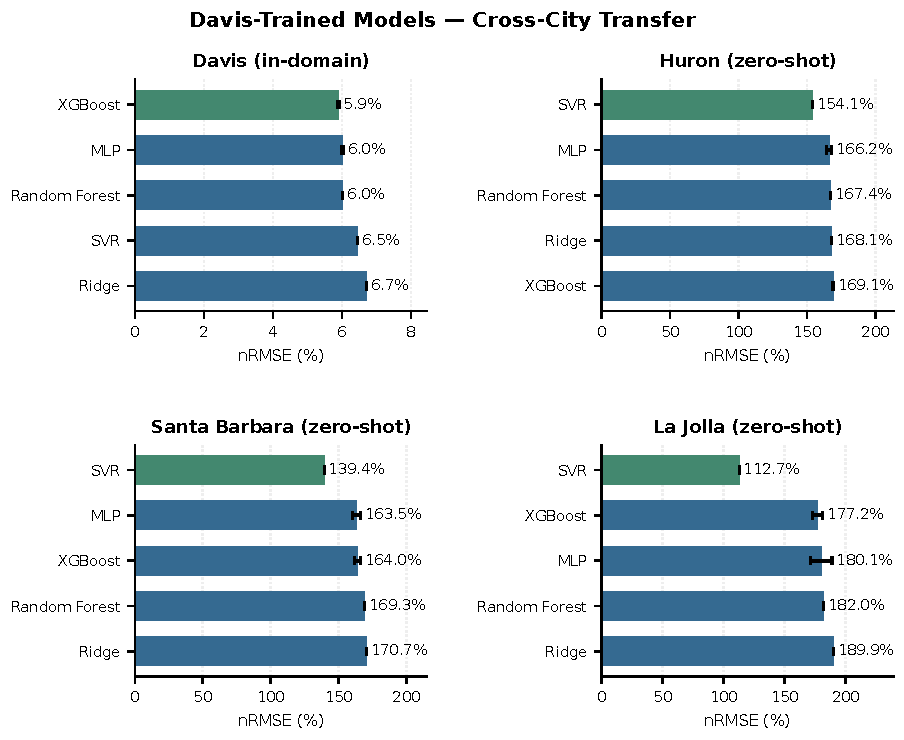
\includegraphics[width=0.93\linewidth,height=5.65cm,keepaspectratio]{Figures/P2/P2_Cross_City_All_Models.pdf}\par
\footeridea{Each plotted model was trained only on Davis, then applied unchanged to every target city (no target-label fitting).}
\note{Now the Davis models are tested, unchanged, in three other cities. At home they reach about
6 percent normalized error. Everywhere else every model is above 100 percent: the error is bigger
than the whole power range of the target city.}
\end{frame}

\begin{frame}{P2 — Why zero-shot fails: PV output scale}
\sectiontag{P2 \quad ANALYSIS — MEASURED MEAN POWER}
\centering
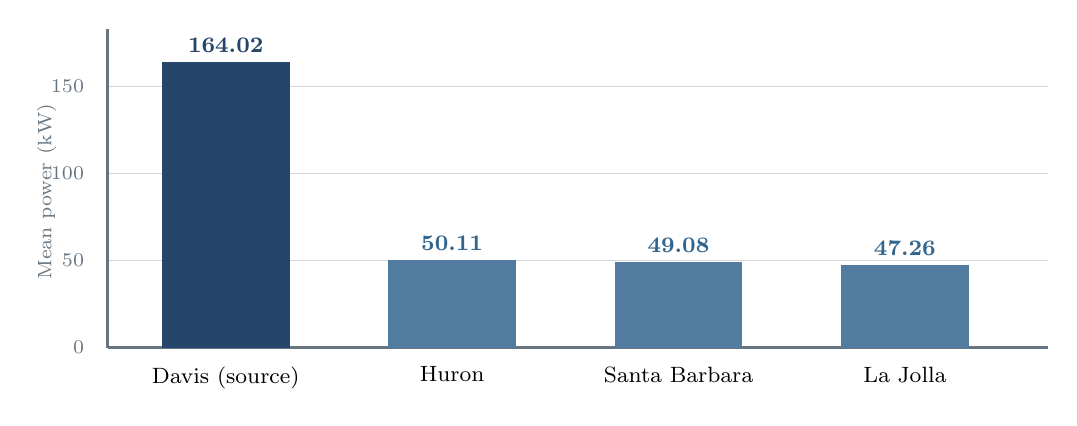
\begin{tikzpicture}[x=1.25cm,y=0.92cm]
  \foreach \yy/\val in {0/0,1.2/50,2.4/100,3.6/150}{
    \draw[slate!28,thin] (0.7,\yy) -- (10.25,\yy);
    \node[font=\scriptsize,text=slate,anchor=east] at (0.56,\yy) {\val};
  }
  \draw[slate,line width=0.8pt] (0.7,0) -- (10.25,0);
  \draw[slate,line width=0.8pt] (0.7,0) -- (0.7,4.4);
  \fill[navy] (1.25,0) rectangle (2.55,3.936);
  \node[font=\footnotesize\bfseries,text=navy,above] at (1.90,3.936) {164.02};
  \fill[teal!85] (3.55,0) rectangle (4.85,1.20264);
  \node[font=\footnotesize\bfseries,text=teal,above] at (4.20,1.20264) {50.11};
  \fill[teal!85] (5.85,0) rectangle (7.15,1.17792);
  \node[font=\footnotesize\bfseries,text=teal,above] at (6.50,1.17792) {49.08};
  \fill[teal!85] (8.15,0) rectangle (9.45,1.13424);
  \node[font=\footnotesize\bfseries,text=teal,above] at (8.80,1.13424) {47.26};
  \node[font=\footnotesize,anchor=north] at (1.90,-0.13) {Davis (source)};
  \node[font=\footnotesize,anchor=north] at (4.20,-0.13) {Huron};
  \node[font=\footnotesize,anchor=north] at (6.50,-0.13) {Santa Barbara};
  \node[font=\footnotesize,anchor=north] at (8.80,-0.13) {La Jolla};
  \node[font=\scriptsize,text=slate,rotate=90] at (0.08,2.15) {Mean power (kW)};
\end{tikzpicture}\par
\vspace{0.08cm}
\smallmuted{Davis produces 3.3--3.5$\times$ more power than the target sites. The models carry this scale with them.}\par
\footeridea{The observed output-scale gap is consistent with large cross-city bias; capacity and weather can also differ.}
\note{The reason is simple. Davis produces on average 164 kilowatts; the other sites produce
about 50. That is more than three times as much. A Davis model has learned Davis's scale and
predicts Davis-sized output everywhere. Keep this in mind for Problem 5.}
\end{frame}



\begin{frame}{P2 — Three vs six years of history}
\sectiontag{P2 \quad RESULTS — HISTORY-LENGTH COMPARISON}
\begin{columns}[T,totalwidth=\textwidth]
\begin{column}{0.62\textwidth}
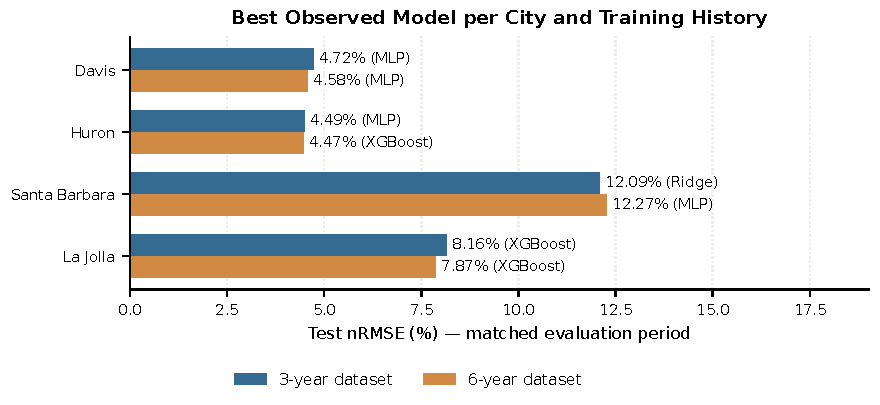
\includegraphics[width=\linewidth,height=5.52cm,keepaspectratio]{Figures/P2/P2_Three_vs_Six_Years_Best_Models.pdf}
\end{column}
\begin{column}{0.34\textwidth}
\factbox{Small, uneven gains}{Best nRMSE, 3\,yr $\to$ 6\,yr:\\
Davis 4.72 $\to$ 4.58\%\\
Huron 4.49 $\to$ 4.47\%\\
La Jolla 8.16 $\to$ 7.87\%\\
Santa Barbara 12.09 $\to$ \textcolor{warn}{12.27\%}}\vspace{0.15cm}
\smallmuted{Best-observed models are selected separately for each history length; this is a descriptive ablation.}
\end{column}
\end{columns}
\footeridea{More history helps three of four cities by at most 0.3 points: far smaller than the cross-city gap.}
\note{Does more history help? A little. Six years improve three of four cities by at most 0.3
percentage points, and Santa Barbara gets slightly worse. Three years may already cover many conditions; the best model can differ between the two lengths. Compared with the cross-city gap, this effect is tiny.}
\end{frame}

\begin{frame}{P2 — Summary: best same-city and sequential models}
\sectiontag{P2 \quad BEST OBSERVED — AFTER ALL-MODEL RESULTS}
\smallmuted{Best observed model within each protocol (three-seed mean); same-city estimates and $K=12$ sequences are different experimental tasks.}
\vspace{0.18cm}
{\small\renewcommand{\arraystretch}{1.35}
\setlength{\tabcolsep}{5pt}
\begin{tabular}{@{}llrrr@{}}\toprule
\textbf{Protocol / city} & \textbf{Best model} & \textbf{RMSE (kW)} & \textbf{MAE (kW)} & \textbf{nRMSE (\%)}\\\midrule
Same-city Davis & XGBoost / MLP & 11.85 & 6.33 / 6.52 & 4.72\\
Same-city Amherst & MLP & 19.96 & 14.09 & 15.69\\\midrule
Sequence Davis ($K=12$) & Random forest & 13.30 & 6.40 & 5.29\\
Sequence Amherst ($K=12$) & Random forest & 15.96 & 10.63 & 12.54\\
\bottomrule\end{tabular}}
\vspace{0.12cm}
\begin{block}{Interpretation}
\footnotesize Classical tree ensembles are competitive with neural models. Random forest beats the LSTM in both sequence tasks. A one-step forecast means the next \emph{recorded} observation; gaps between daily recording windows may change the elapsed time.
\end{block}
\note{Complete model tables and the history comparison are in the written report. The best same-city models are XGBoost and MLP, with almost identical Davis RMSE. In Amherst the MLP leads. In the history-based task, random forest wins both sites, not the LSTM. The time between two recorded rows is normally 30 minutes during the window, but can include overnight gaps.}
\end{frame}

\begin{frame}{P2 — Results: prediction traces}
\sectiontag{P2 \quad RESULTS — PREDICTION VS TRUTH}
\vspace{-0.06cm}
\begin{columns}[T,totalwidth=\textwidth]
\begin{column}{0.49\textwidth}
\centering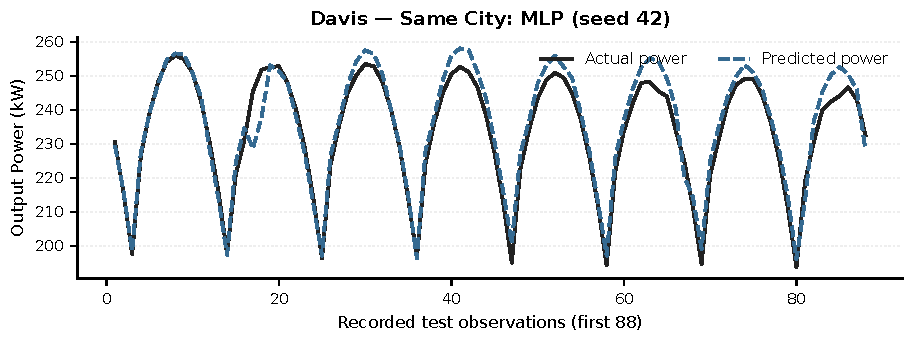
\includegraphics[width=\linewidth,height=3.50cm,keepaspectratio]{Figures/P2/P2_Same_City_Davis_Prediction_Trace.pdf}
\par{\scriptsize Davis: MLP, same-city prediction}
\end{column}
\begin{column}{0.49\textwidth}
\centering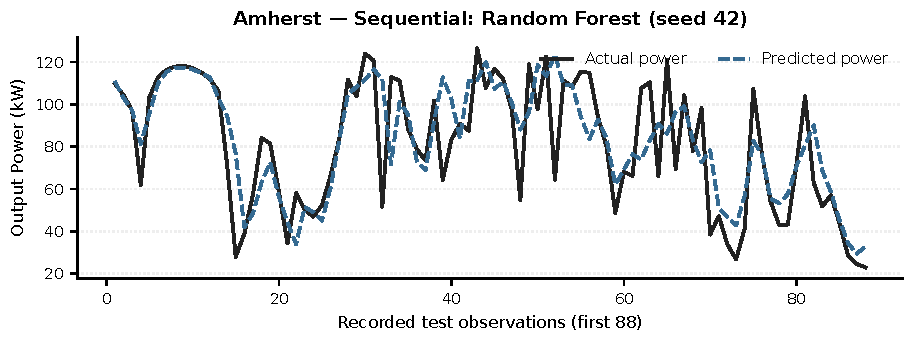
\includegraphics[width=\linewidth,height=3.50cm,keepaspectratio]{Figures/P2/P2_Sequential_Amherst_Prediction_Trace.pdf}
\par{\scriptsize Amherst: random forest, next-step forecast}
\end{column}
\end{columns}
\vspace{0.08cm}
{\footnotesize
\renewcommand{\arraystretch}{1.18}
\setlength{\tabcolsep}{5pt}
\begin{tabularx}{\linewidth}{@{}Xrrr@{}}\toprule
\textbf{Held-out test (seed 42)} & \textbf{RMSE (kW)} & \textbf{MAE (kW)} & \textbf{nRMSE (\%)}\\\midrule
Davis --- MLP (same-city) & 11.63 & 6.29 & 4.63\\
Amherst --- RF (sequential) & 15.95 & 10.63 & 12.54\\
\bottomrule\end{tabularx}
}
\footeridea{Predictions follow the daily shape; the largest misses are fast ramps from passing clouds.}
\note{These traces show prediction versus truth on the test period. The models follow the daily
shape well; large misses can occur on rapid irradiance changes; elapsed time can vary across day boundaries.}
\end{frame}

\section{P3: Dimensionality Reduction}

\begin{frame}{Problem 3 — Dimension Reduction for Prediction}
\sectiontag{P3 \quad PROBLEM}
\begin{block}{Objective from the assignment}
Compress the irradiance and weather features into a lower-dimensional representation, \textbf{then use it for P1 classification and P2 regression}.
\end{block}
\begin{columns}[T,totalwidth=\textwidth]
\begin{column}{0.49\textwidth}
\begin{block}{Task A: Learn compressed inputs}
Unsupervised reduction to $d\in\{2,5,10\}$; labels are never used to fit the reducer.
\end{block}
\end{column}
\begin{column}{0.49\textwidth}
\begin{block}{Task B: Compare predictions}
Train classifier/regressor on reduced features; compare with the same model on full features.
\end{block}
\end{column}
\end{columns}
\vspace{0.10cm}
\factbox{Deliverable in the question}{Explained variance, reconstruction error, downstream accuracy/RMSE/MAE, and a 2D t-SNE / UMAP visualization.}
\note{Problem 3 asks whether we can compress the inputs to 2, 5 or 10 dimensions without labels and
still predict well. The reducer never sees labels; its value is judged by how well a downstream
model does on the compressed features.}
\end{frame}

\begin{frame}{P3 — Reduction methods and downstream models}
\sectiontag{P3 \quad MODELS}
\renewcommand{\arraystretch}{1.34}
\begin{tabularx}{\linewidth}{@{}P{2.2cm}YP{3.15cm}@{}}\toprule
\textbf{Family} & \textbf{Representations / predictors} & \textbf{Implementation}\\\midrule
\rowcolor{softblue} Classical unsupervised & Linear PCA; RBF Kernel PCA (Nystr\"om, 192 landmarks) & scikit-learn\\
\rowcolor{softteal} Deep unsupervised & Autoencoder $p\to64\to32\to d$, symmetric decoder & PyTorch\\
\rowcolor{softblue} Classical downstream & Logistic / SVM / RF / XGBoost; Ridge / SVR / RF / XGBoost & scikit-learn, XGBoost\\
\rowcolor{softteal} Deep downstream & Classification and regression MLPs & PyTorch\\\bottomrule
\end{tabularx}\par
\vspace{0.18cm}
\smallmuted{The autoencoder minimizes input-reconstruction error; t-SNE and UMAP are used only for 2D visualization.}
\note{I compare linear PCA, an approximate RBF kernel PCA, and a neural autoencoder. On top of
each, the same five classifiers and regressors from P1 and P2 are trained.}
\end{frame}

\begin{frame}{P3 — Intrinsic quality: variance and reconstruction}
\sectiontag{P3 \quad RESULTS — INTRINSIC}
\begin{columns}[T,totalwidth=\textwidth]
\begin{column}{0.49\textwidth}
\centering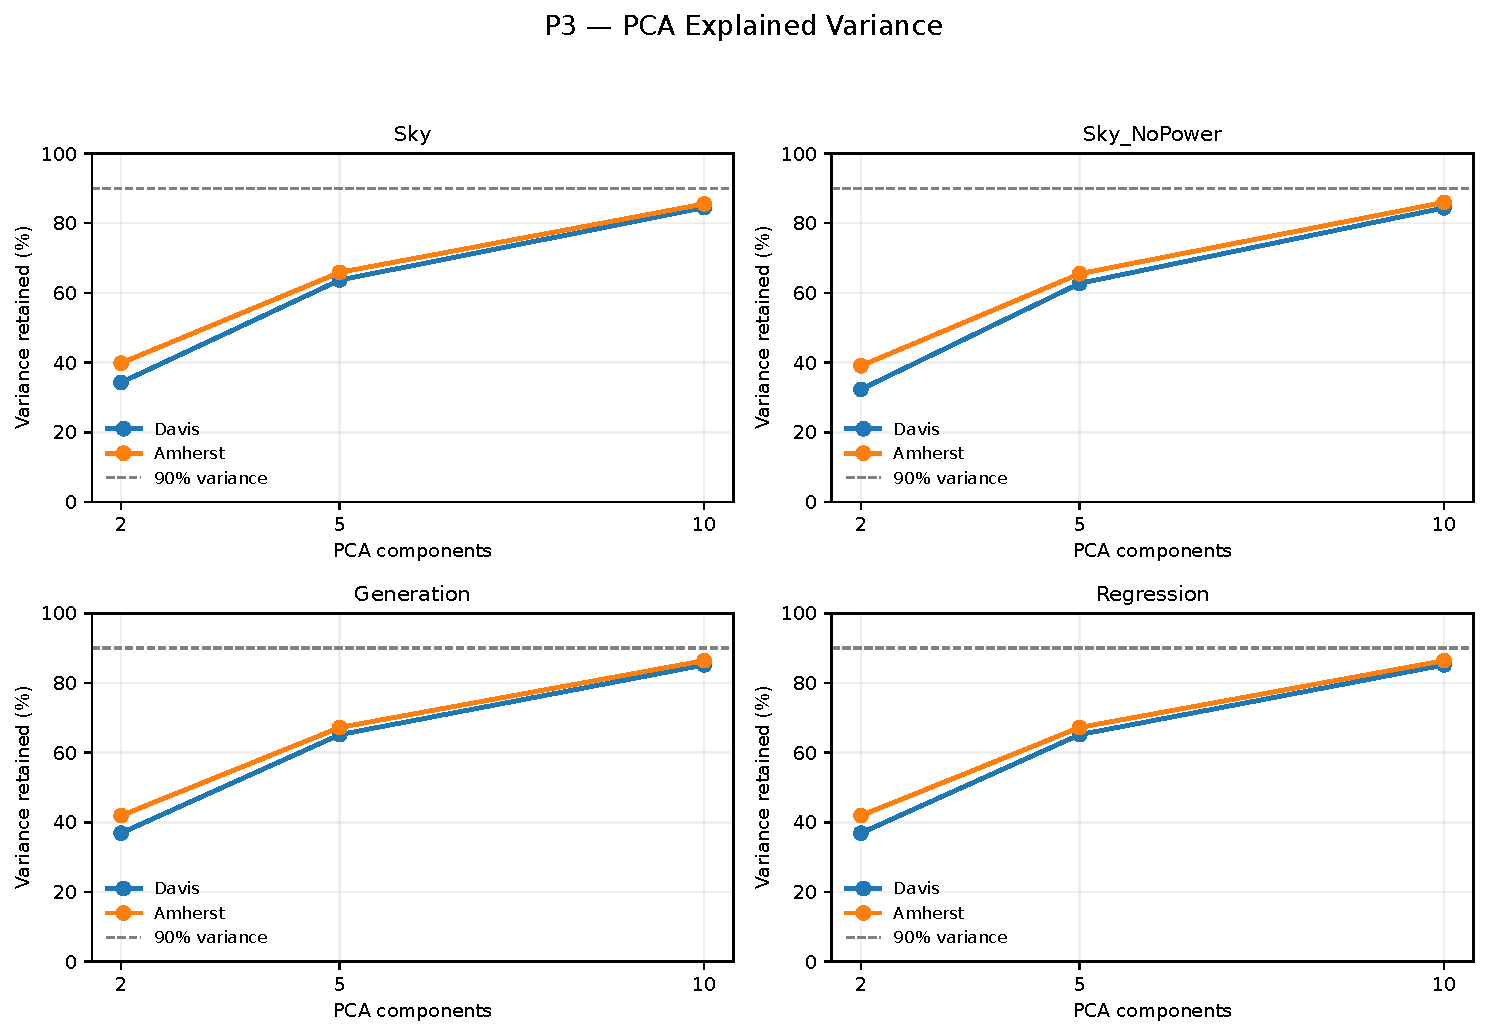
\includegraphics[width=\linewidth,height=5.12cm,keepaspectratio]{Figures/P3/P3_Final_PCA_Explained_Variance.pdf}
\smallmuted{PCA cumulative explained variance}
\end{column}
\begin{column}{0.49\textwidth}
\centering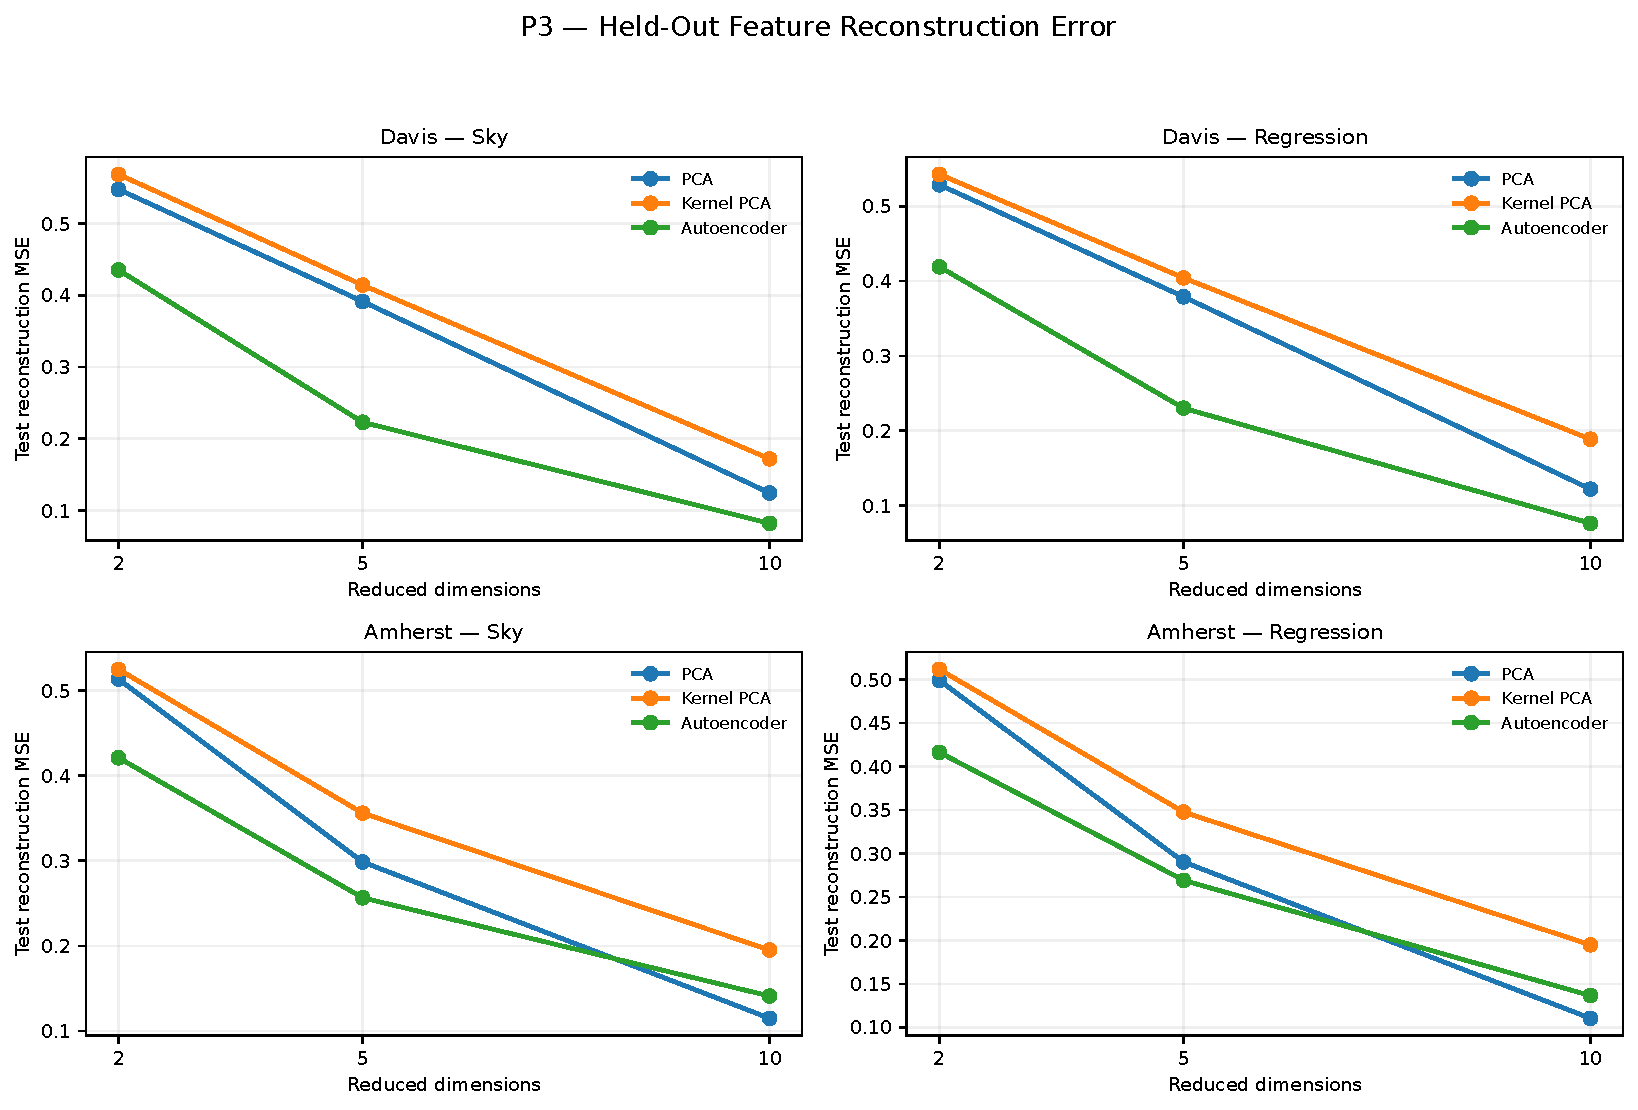
\includegraphics[width=\linewidth,height=5.12cm,keepaspectratio]{Figures/P3/P3_Final_Reconstruction_Comparison.pdf}
\smallmuted{Held-out reconstruction MSE}
\end{column}
\end{columns}
\footeridea{The autoencoder reconstructs best at small $d$; ten PCA components keep 84--86\% of the variance.}
\note{On the left, PCA's explained variance; on the right, test reconstruction error. More
components keep more information, and the autoencoder reconstructs best at small bottlenecks. Ten
PCA components keep about 85 percent of the variance.}
\end{frame}

\begin{frame}{P3 — Downstream models: sky-condition classification}
\sectiontag{P3 \quad RESULTS — 10-DIMENSIONAL INPUTS}
\smallmuted{Same classifier held fixed within each row: compare PCA vs Kernel PCA vs AE at $d=10$. BA (\%), three-seed mean. \emph{Raw best} is a separate overall leaderboard, not the same-model baseline.}\vspace{0.18cm}
\begin{columns}[T,onlytextwidth]
\begin{column}{0.486\textwidth}
\textbf{Davis}\hfill{\scriptsize raw best: 99.17}\par\vspace{0.12cm}
{\fontsize{8.8}{10.4}\selectfont
\setlength{\tabcolsep}{3.9pt}
\renewcommand{\arraystretch}{1.39}
\begin{tabular}{@{}lrrr@{}}\toprule
\textbf{Model} & \textbf{PCA} & \textbf{KPCA} & \textbf{AE}\\\midrule
Logistic & 80.40 & 80.36 & 83.28\\
RBF SVM & 78.91 & 81.83 & \textcolor{teal}{\textbf{84.40}}\\
RF & 80.51 & 81.86 & 81.64\\
XGBoost & 81.09 & 81.23 & 82.69\\
MLP & 81.66 & 81.99 & 84.08\\
\bottomrule\end{tabular}}
\end{column}
\begin{column}{0.486\textwidth}
\textbf{Amherst}\hfill{\scriptsize raw best: 98.98}\par\vspace{0.12cm}
{\fontsize{8.8}{10.4}\selectfont
\setlength{\tabcolsep}{3.9pt}
\renewcommand{\arraystretch}{1.39}
\begin{tabular}{@{}lrrr@{}}\toprule
\textbf{Model} & \textbf{PCA} & \textbf{KPCA} & \textbf{AE}\\\midrule
Logistic & 86.64 & 84.03 & 81.95\\
RBF SVM & \textcolor{teal}{\textbf{88.19}} & 85.18 & 84.23\\
RF & 85.01 & 83.75 & 81.57\\
XGBoost & 86.27 & 84.04 & 81.22\\
MLP & 87.68 & 85.31 & 82.35\\
\bottomrule\end{tabular}}
\end{column}
\end{columns}
\vspace{0.30cm}
\begin{beamercolorbox}[wd=\linewidth,sep=0.14cm]{block body}
\footnotesize \textcolor{teal}{\textbf{Teal}} = best compressed configuration at $d=10$. Full $d=2,5,10$ tables are in the report.
\end{beamercolorbox}
\note{At ten dimensions, the best compressed sky classifier reaches 84.4 percent in Davis and 88.2
in Amherst, compared with about 99 percent on raw features.}
\end{frame}

\begin{frame}{P3 — Downstream models: sky without Output Power}
\sectiontag{P3 \quad RESULTS — 10-DIMENSIONAL INPUTS}
\smallmuted{Same classifier held fixed within each row: compare PCA vs Kernel PCA vs AE at $d=10$. BA (\%), three-seed mean. \emph{Raw best} is a separate overall leaderboard, not the same-model baseline.}\vspace{0.18cm}
\begin{columns}[T,onlytextwidth]
\begin{column}{0.486\textwidth}
\textbf{Davis}\hfill{\scriptsize raw best: 99.20}\par\vspace{0.12cm}
{\fontsize{8.8}{10.4}\selectfont
\setlength{\tabcolsep}{3.9pt}
\renewcommand{\arraystretch}{1.39}
\begin{tabular}{@{}lrrr@{}}\toprule
\textbf{Model} & \textbf{PCA} & \textbf{KPCA} & \textbf{AE}\\\midrule
Logistic & 80.35 & 78.80 & 81.87\\
RBF SVM & 78.55 & 81.90 & \textcolor{teal}{\textbf{84.19}}\\
RF & 79.28 & 79.92 & 79.22\\
XGBoost & 81.02 & 80.19 & 81.97\\
MLP & 80.50 & 81.67 & 83.96\\
\bottomrule\end{tabular}}
\end{column}
\begin{column}{0.486\textwidth}
\textbf{Amherst}\hfill{\scriptsize raw best: 98.96}\par\vspace{0.12cm}
{\fontsize{8.8}{10.4}\selectfont
\setlength{\tabcolsep}{3.9pt}
\renewcommand{\arraystretch}{1.39}
\begin{tabular}{@{}lrrr@{}}\toprule
\textbf{Model} & \textbf{PCA} & \textbf{KPCA} & \textbf{AE}\\\midrule
Logistic & 86.23 & 81.75 & 81.02\\
RBF SVM & \textcolor{teal}{\textbf{87.60}} & 86.23 & 83.97\\
RF & 84.63 & 83.39 & 81.09\\
XGBoost & 85.86 & 83.68 & 81.52\\
MLP & 87.20 & 85.34 & 82.96\\
\bottomrule\end{tabular}}
\end{column}
\end{columns}
\vspace{0.30cm}
\begin{beamercolorbox}[wd=\linewidth,sep=0.14cm]{block body}
\footnotesize Removing Output Power changes the raw score by $\le$0.03 points: power is not the shortcut for the sky label.
\end{beamercolorbox}
\note{Removing Output Power from the sky inputs barely changes anything, either raw or compressed.
So the sky classifier is not secretly reading the power column.}
\end{frame}

\begin{frame}{P3 — Downstream models: generation-regime classification}
\sectiontag{P3 \quad RESULTS — 10-DIMENSIONAL INPUTS}
\smallmuted{Same classifier held fixed within each row: compare PCA vs Kernel PCA vs AE at $d=10$. BA (\%), three-seed mean. \emph{Raw best} is a separate overall leaderboard, not the same-model baseline.}\vspace{0.18cm}
\begin{columns}[T,onlytextwidth]
\begin{column}{0.486\textwidth}
\textbf{Davis}\hfill{\scriptsize raw best: 94.50}\par\vspace{0.12cm}
{\fontsize{8.8}{10.4}\selectfont
\setlength{\tabcolsep}{3.9pt}
\renewcommand{\arraystretch}{1.39}
\begin{tabular}{@{}lrrr@{}}\toprule
\textbf{Model} & \textbf{PCA} & \textbf{KPCA} & \textbf{AE}\\\midrule
Logistic & 85.90 & 86.82 & 84.33\\
RBF SVM & 88.94 & 88.72 & 87.61\\
RF & \textcolor{teal}{\textbf{89.45}} & 88.78 & 86.07\\
XGBoost & 88.93 & 88.34 & 86.08\\
MLP & 88.17 & 86.85 & 88.77\\
\bottomrule\end{tabular}}
\end{column}
\begin{column}{0.486\textwidth}
\textbf{Amherst}\hfill{\scriptsize raw best: 76.06}\par\vspace{0.12cm}
{\fontsize{8.8}{10.4}\selectfont
\setlength{\tabcolsep}{3.9pt}
\renewcommand{\arraystretch}{1.39}
\begin{tabular}{@{}lrrr@{}}\toprule
\textbf{Model} & \textbf{PCA} & \textbf{KPCA} & \textbf{AE}\\\midrule
Logistic & 73.91 & 74.20 & 74.62\\
RBF SVM & 73.21 & 74.68 & 75.29\\
RF & 73.36 & \textcolor{teal}{\textbf{75.56}} & 73.68\\
XGBoost & 74.41 & 75.14 & 73.97\\
MLP & 73.84 & 75.06 & 74.63\\
\bottomrule\end{tabular}}
\end{column}
\end{columns}
\vspace{0.30cm}
\begin{beamercolorbox}[wd=\linewidth,sep=0.14cm]{block body}
\footnotesize Amherst generation loses only 0.5 points at $d=10$: when the raw model is already limited by missing information, compression costs little. (Davis best overall: PCA $d=5$, 90.62\%.)
\end{beamercolorbox}
\note{For generation regimes the penalty is smaller. In Amherst, kernel PCA with ten components is
only half a point below raw features. When the full model is already limited by information that is
not in the inputs, removing redundant dimensions costs very little.}
\end{frame}

\begin{frame}{P3 — Downstream models: PV power regression}
\sectiontag{P3 \quad RESULTS — 10-DIMENSIONAL INPUTS}
\smallmuted{Same regressor held fixed within each row: compare PCA vs Kernel PCA vs AE at $d=10$. RMSE (kW), three-seed mean. \emph{Raw best} is a separate overall leaderboard.}\vspace{0.18cm}
\begin{columns}[T,onlytextwidth]
\begin{column}{0.486\textwidth}
\textbf{Davis}\hfill{\scriptsize raw best: 14.93}\par\vspace{0.12cm}
{\fontsize{8.8}{10.4}\selectfont
\setlength{\tabcolsep}{3.9pt}
\renewcommand{\arraystretch}{1.39}
\begin{tabular}{@{}lrrr@{}}\toprule
\textbf{Model} & \textbf{PCA} & \textbf{KPCA} & \textbf{AE}\\\midrule
Ridge & 24.09 & 26.63 & 22.44\\
RBF SVR & 27.98 & 24.32 & \textcolor{teal}{\textbf{17.85}}\\
RF & 20.09 & 20.68 & 20.35\\
XGBoost & 21.09 & 20.54 & 21.24\\
MLP & 20.01 & 20.36 & 17.86\\
\bottomrule\end{tabular}}
\end{column}
\begin{column}{0.486\textwidth}
\textbf{Amherst}\hfill{\scriptsize raw best: 19.97}\par\vspace{0.12cm}
{\fontsize{8.8}{10.4}\selectfont
\setlength{\tabcolsep}{3.9pt}
\renewcommand{\arraystretch}{1.39}
\begin{tabular}{@{}lrrr@{}}\toprule
\textbf{Model} & \textbf{PCA} & \textbf{KPCA} & \textbf{AE}\\\midrule
Ridge & 21.42 & 20.98 & 21.47\\
RBF SVR & 23.39 & 21.53 & 20.53\\
RF & 20.92 & 20.92 & 20.95\\
XGBoost & 20.90 & 20.91 & 20.75\\
MLP & 20.69 & \textcolor{teal}{\textbf{20.25}} & 20.45\\
\bottomrule\end{tabular}}
\end{column}
\end{columns}
\vspace{0.30cm}
\begin{beamercolorbox}[wd=\linewidth,sep=0.14cm]{block body}
\footnotesize In Davis the non-linear autoencoder gives the best compressed regressors (SVR and MLP, $\approx$17.9\,kW).
\end{beamercolorbox}
\note{The detailed regression table: in Davis both the best and second-best compressed regressors use
autoencoder features, so a non-linear bottleneck keeps more of the power-relevant information.}
\end{frame}

\begin{frame}{P3 — Controlled comparison: same downstream model}
\sectiontag{P3 \quad RESULTS — WHAT CHANGES, WHAT STAYS FIXED}
\smallmuted{\textbf{Hold predictor and $d=10$ fixed}; vary only the feature representation. Original features are uncompressed. Three-seed test means.}
\vspace{0.20cm}
\begin{columns}[T,totalwidth=\textwidth]
\begin{column}{0.49\textwidth}
\textbf{Sky: fixed RBF SVM}\par\smallmuted{Balanced accuracy (\%), higher is better.}
{\footnotesize\setlength{\tabcolsep}{5.0pt}\renewcommand{\arraystretch}{1.35}
\begin{tabular}{@{}lrr@{}}\toprule
\textbf{Input} & \textbf{Davis} & \textbf{Amherst}\\\midrule
Original & \textcolor{teal}{\textbf{97.52}} & \textcolor{teal}{\textbf{96.36}}\\
PCA & 78.91 & 88.19\\
Kernel PCA & 81.83 & 85.18\\
Autoencoder & 84.40 & 84.23\\
\bottomrule\end{tabular}}
\end{column}
\begin{column}{0.49\textwidth}
\textbf{Power: fixed RBF SVR}\par\smallmuted{RMSE (kW), lower is better.}
{\footnotesize\setlength{\tabcolsep}{5.0pt}\renewcommand{\arraystretch}{1.35}
\begin{tabular}{@{}lrr@{}}\toprule
\textbf{Input} & \textbf{Davis} & \textbf{Amherst}\\\midrule
Original & \textcolor{teal}{\textbf{17.36}} & 27.07\\
PCA & 27.98 & 23.39\\
Kernel PCA & 24.32 & 21.53\\
Autoencoder & 17.85 & \textcolor{teal}{\textbf{20.53}}\\
\bottomrule\end{tabular}}
\end{column}
\end{columns}
\vspace{0.06cm}
\smallmuted{\textbf{Interpretation:} Within each task, the prediction model stays fixed, so only the representation changes. Compression may improve an individual regressor (e.g., Amherst SVR) without winning the best-overall leaderboard.}
\note{This is the controlled comparison missing from the original deck. We hold the downstream model fixed: RBF SVM for Sky and RBF SVR for regression, using the same train-test split. In Amherst, SVR can actually improve with compression, even though the best model across all raw features still wins the overall leaderboard. Comparing best combinations and controlled comparisons answers two distinct questions.}
\end{frame}

\begin{frame}{P3 — Extra metrics: accuracy and MAE at 10D (Davis)}
\sectiontag{P3 \quad SUPPLEMENTARY METRICS — BEST MODELS PER INPUT}
\begin{columns}[T,totalwidth=\textwidth]
\begin{column}{0.49\textwidth}
\textbf{Sky classification} {\scriptsize(\%)}\par\vspace{0.13cm}
{\footnotesize\begin{tabular}{@{}lrr@{}}\toprule
\textbf{Input} & \textbf{Accuracy} & \textbf{Balanced Acc.}\\\midrule
Original & 99.3 & 99.2 \\
PCA 10D & 87.7 & 81.7 \\
Kernel PCA 10D & 87.2 & 82.0 \\
Autoencoder 10D & 89.6 & 84.4 \\
\bottomrule\end{tabular}}\par
\end{column}
\begin{column}{0.49\textwidth}
\textbf{Power regression} {\scriptsize(kW)}\par\vspace{0.13cm}
{\footnotesize\begin{tabular}{@{}lrr@{}}\toprule
\textbf{Input} & \textbf{RMSE} & \textbf{MAE}\\\midrule
Original & 14.93 & 8.71 \\
PCA 10D & 20.01 & 12.46 \\
Kernel PCA 10D & 20.36 & 13.84 \\
Autoencoder 10D & 17.85 & 11.20 \\
\bottomrule\end{tabular}}\par
\end{column}
\end{columns}
\vspace{0.35cm}
\begin{beamercolorbox}[sep=0.15cm,wd=\linewidth]{block body}
\footnotesize \textbf{Best model selected independently for each representation} (not a fixed-classifier test). Accuracy is higher than BA after compression because errors concentrate in smaller classes.
\end{beamercolorbox}
\note{The assignment also asks for plain accuracy and MAE. They tell the same story. Note that after
compression accuracy is higher than balanced accuracy: the errors fall disproportionately on the
smaller classes.}
\end{frame}

\begin{frame}{P3 — Summary: best compression across 2, 5 and 10D}
\sectiontag{P3 \quad RESULTS — BEST OF $d=2,5,10$}
\smallmuted{\textbf{Best-combination comparison:} choose the reducer, dimension $d$, and downstream model separately for each city/task. These are NOT fixed-classifier comparisons.}\par\vspace{0.12cm}
{\fontsize{8.0}{9.5}\selectfont
\setlength{\tabcolsep}{3.9pt}\renewcommand{\arraystretch}{1.28}
\begin{tabular}{@{}lllrlrrr@{}}\toprule
\textbf{City} & \textbf{Task} & \textbf{Method} & \textbf{d} & \textbf{Best model} & \textbf{Reduced} & \textbf{Raw best} & \shortstack{\textbf{Loss vs}\\\textbf{raw}}\\\midrule
Davis & Sky & AE & 10 & RBF SVM & 84.40 & 99.17 & \textcolor{warn}{$+14.77$}\\
Davis & Sky-NoPower & AE & 10 & RBF SVM & 84.19 & 99.20 & \textcolor{warn}{$+15.01$}\\
Davis & Generation & PCA & 5 & RBF SVM & 90.62 & 94.50 & $+3.88$\\
Davis & Regression & AE & 10 & RBF SVR & 17.85 & 14.93 & $+2.92$\,kW\\
\midrule
Amherst & Sky & PCA & 10 & RBF SVM & 88.19 & 98.98 & \textcolor{warn}{$+10.79$}\\
Amherst & Sky-NoPower & PCA & 10 & RBF SVM & 87.60 & 98.96 & \textcolor{warn}{$+11.36$}\\
Amherst & Generation & KPCA & 10 & RF & \textbf{75.56} & 76.06 & $+0.50$\\
Amherst & Regression & KPCA & 10 & MLP & \textbf{20.25} & 19.97 & $+0.28$\,kW\\
\bottomrule\end{tabular}}\par\vspace{0.18cm}
\smallmuted{Classification loss = Raw BA $-$ Reduced BA (percentage points); regression loss = Reduced RMSE $-$ Raw RMSE (kW). All loss values are positive: \textbf{raw wins 8/8}. Models may differ between best raw and best reduced.}
\note{Here, model selection is allowed to vary over reducer, dimension and downstream classifier/regressor. Raw-feature leaders can be different models. Raw wins all eight best-vs-best comparisons. The loss is largest for
the sky label, ten to fifteen points, and smallest for Amherst generation and regression.}
\end{frame}

\begin{frame}{P3 — Analysis: why compression hurts the sky task}
\sectiontag{P3 \quad ANALYSIS}
\begin{columns}[T,totalwidth=\textwidth]
\begin{column}{0.52\textwidth}
\centering
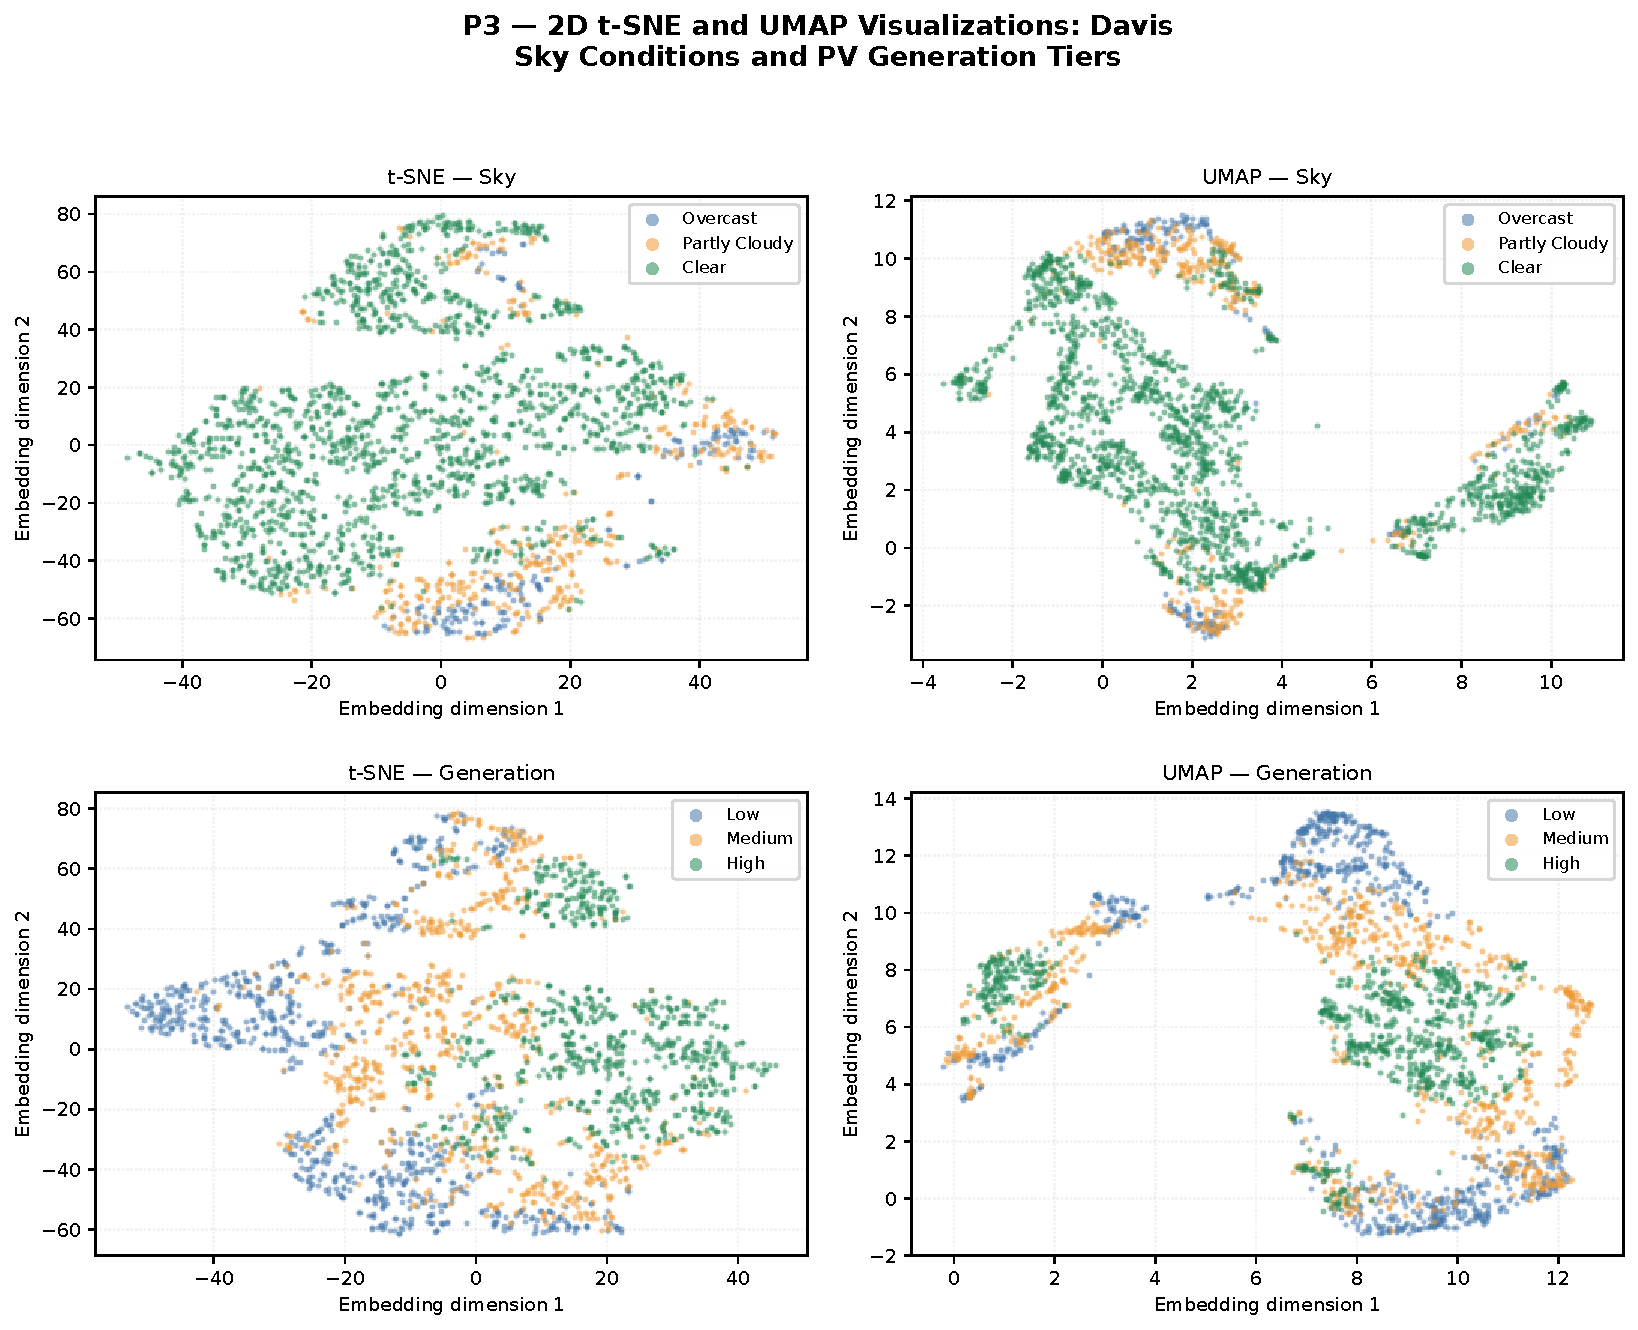
\includegraphics[width=\linewidth,height=4.93cm,keepaspectratio]{Figures/P3/P3_2D_tSNE_UMAP_Davis.pdf}
\smallmuted{Davis: 2D class-colored t-SNE / UMAP maps}
\end{column}
\begin{column}{0.45\textwidth}
\begin{itemize}\setlength\itemsep{0.36em}\small
\item \textbf{PCA keeps variance, not labels.} The sky label is a narrow irradiance \emph{ratio}; most input variance is temperature, humidity, wind and time.
\item Non-linear AE helps most at tight bottlenecks.
\item 2D maps separate sky classes and order Low$\to$Medium$\to$High, but maps are not accuracy.
\end{itemize}
\end{column}
\end{columns}
\footeridea{Unsupervised compression is a trade-off: smaller inputs, less label information.}
\note{Why does compression hurt the sky task so much? PCA keeps the directions of largest variance,
but the sky label is a ratio of two irradiance columns, while most of the variance comes from
temperature, humidity, wind and time. So the label signal is spread thinly across components. The
t-SNE and UMAP maps do show clear sky clusters, but a nice map is not a good classifier.}
\end{frame}



\section{P4: Semi-supervised Learning}

\begin{frame}{Problem 4 — Semi-Supervised Learning}
\sectiontag{P4 \quad PROBLEM}
\begin{block}{Objective from the assignment}
Learn when \textbf{only a fraction of training labels is available} while keeping the unlabeled majority useful.
\end{block}
\begin{columns}[T,totalwidth=\textwidth]
\begin{column}{0.49\textwidth}
\begin{block}{Task A: Withhold labels}
Only $p\in\{10\%,30\%,50\%\}$ of training observations keep their labels.
\end{block}
\end{column}
\begin{column}{0.49\textwidth}
\begin{block}{Task B: Matched evaluation}
SSL and supervised-only models use the \textbf{same labeled subset}; both are tested on the full test set.
\end{block}
\end{column}
\end{columns}
\vspace{0.10cm}
\factbox{Deliverable in the question}{Label-efficiency curve and the SSL gain over supervised-only --- especially: can SSL win at 10\% labels?}
\note{Problem 4 simulates failed sensors: only 10, 30 or 50 percent of training labels are kept.
The key question is whether the unlabeled rest helps, compared with a supervised model trained on
exactly the same labeled subset.}
\end{frame}

\begin{frame}{P4 — Models and SSL strategies}
\sectiontag{P4 \quad MODELS}
\renewcommand{\arraystretch}{1.30}
{\small
\begin{tabularx}{\linewidth}{@{}P{3.6cm}Y@{}}\toprule
\textbf{Strategy} & \textbf{How it uses unlabeled data}\\\midrule
\rowcolor{softblue} Supervised-only & Ignores it (baseline)\\
\rowcolor{softgold} One-shot pseudo-labeling & Model labels the unlabeled pool once; refit on labeled + pseudo-labeled\\
\rowcolor{softgold} Iterative self-training & Repeat: add confident pseudo-labels, refit, over several rounds\\
\rowcolor{softteal} Autoencoder SSL & Learn features from \emph{all} training inputs; classify with labeled subset\\\bottomrule
\end{tabularx}\par}
\vspace{0.15cm}
\smallmuted{Each strategy is applied to all five classifiers: logistic regression, RBF SVM, random forest, XGBoost, PyTorch MLP $\Rightarrow$ 20 combinations per task and budget.}
\note{I compare four strategies. Supervised-only ignores unlabeled data. One-shot pseudo-labeling
labels the pool once and refits. Iterative self-training repeats that with confident predictions.
Autoencoder SSL learns features from all inputs and then trains the classifier on the labeled part.
Each strategy is combined with all five classifiers.}
\end{frame}

\begin{frame}{P4 — All classifiers: Davis at 10\% labels}
\sectiontag{P4 \quad RESULTS — SUPERVISED VS SEMI-SUPERVISED}
\smallmuted{Balanced accuracy (\%, three-seed mean). SSL = best observed one-shot, iterative or AE strategy for the same base model.}
\vspace{0.15cm}
{\fontsize{8.6}{10.3}\selectfont
\setlength{\tabcolsep}{4.5pt}
\renewcommand{\arraystretch}{1.35}
\centering
\begin{tabular}{@{}lrrlrrl@{}}\toprule
 & \multicolumn{3}{c}{\textbf{Sky}} & \multicolumn{3}{c}{\textbf{Generation}}\\\cmidrule(lr){2-4}\cmidrule(l){5-7}
\textbf{Base model} & \textbf{Sup.} & \textbf{SSL} & \textbf{Method} & \textbf{Sup.} & \textbf{SSL} & \textbf{Method}\\\midrule
Logistic & 95.77 & 95.65 & AE & 92.10 & 91.90 & Iterative\\
RBF SVM & 91.73 & 91.69 & AE & 91.03 & 91.11 & Iterative\\
Random forest & 97.54 & 97.63 & Iterative & 94.39 & 94.38 & Iterative\\
XGBoost & \textcolor{teal}{\textbf{97.92}} & 97.86 & AE & 94.63 & \textcolor{teal}{\textbf{94.71}} & One-shot\\
MLP & 92.27 & 93.30 & Iterative & 85.55 & 91.14 & AE\\
\bottomrule\end{tabular}\par}
\vspace{0.10cm}
\smallmuted{Same classifier within each row; best SSL strategy is selected descriptively from held-out test results (not a validation-selected winner).}
\footeridea{The strongest baseline is already good; unlabeled data helps some models, but not consistently.}
\note{Here are the results for all five classifiers, not just a single best model. Each classifier has a supervised-only reference and its strongest observed semi-supervised variant. The best strategy varies with model, city and task, so there is no universal SSL winner. The 30 and 50 percent results appear in the label-efficiency plots and the report.}
\end{frame}

\begin{frame}{P4 — All classifiers: Amherst at 10\% labels}
\sectiontag{P4 \quad RESULTS — SUPERVISED VS SEMI-SUPERVISED}
\smallmuted{Balanced accuracy (\%, three-seed mean). SSL = best observed one-shot, iterative or AE strategy for the same base model.}
\vspace{0.15cm}
{\fontsize{8.6}{10.3}\selectfont
\setlength{\tabcolsep}{4.5pt}
\renewcommand{\arraystretch}{1.35}
\centering
\begin{tabular}{@{}lrrlrrl@{}}\toprule
 & \multicolumn{3}{c}{\textbf{Sky}} & \multicolumn{3}{c}{\textbf{Generation}}\\\cmidrule(lr){2-4}\cmidrule(l){5-7}
\textbf{Base model} & \textbf{Sup.} & \textbf{SSL} & \textbf{Method} & \textbf{Sup.} & \textbf{SSL} & \textbf{Method}\\\midrule
Logistic & 97.06 & 97.05 & Iterative & 73.48 & 73.84 & AE\\
RBF SVM & 92.76 & 92.82 & AE & 69.99 & 70.03 & Iterative\\
Random forest & 97.65 & 97.65 & One-shot & 74.46 & \textcolor{teal}{\textbf{74.62}} & Iterative\\
XGBoost & 97.79 & \textcolor{teal}{\textbf{97.88}} & One-shot & 74.09 & 74.33 & Iterative\\
MLP & 95.68 & 96.22 & Iterative & 74.02 & 74.05 & One-shot\\
\bottomrule\end{tabular}\par}
\vspace{0.10cm}
\smallmuted{Same classifier within each row; best SSL strategy is selected descriptively from held-out test results (not a validation-selected winner).}
\footeridea{The strongest baseline is already good; unlabeled data helps some models, but not consistently.}
\note{Here are the results for all five classifiers, not just a single best model. Each classifier has a supervised-only reference and its strongest observed semi-supervised variant. The best strategy varies with model, city and task, so there is no universal SSL winner. The 30 and 50 percent results appear in the label-efficiency plots and the report.}
\end{frame}

\begin{frame}{P4 — Fixed XGBoost: Sky across label budgets}
\sectiontag{P4 \quad CONTROLLED SSL COMPARISON — ONE CLASSIFIER}
\smallmuted{\textbf{Fixed:} XGBoost classifier, city/task, labeled subsets, splits and seeds. \textbf{Varied:} training strategy. BA (\%) over three seeds; higher is better.}
\vspace{0.20cm}
\begin{columns}[T,totalwidth=\textwidth]
\begin{column}{0.49\textwidth}
\textbf{Davis — Sky}\par\vspace{0.10cm}
{\fontsize{8.2}{9.6}\selectfont\setlength{\tabcolsep}{2.9pt}\renewcommand{\arraystretch}{1.40}
\begin{tabular}{@{}rrrrr@{}}\toprule
\textbf{Labels} & \textbf{Sup.} & \textbf{One-shot} & \textbf{Iter.} & \textbf{AE SSL}\\\midrule
10\% & \textcolor{teal}{\textbf{97.92}} & 97.67 & 97.72 & 97.86\\
30\% & 98.72 & 98.28 & \textcolor{teal}{\textbf{98.74}} & 98.53\\
50\% & \textcolor{teal}{\textbf{99.14}} & 99.07 & 99.03 & 98.91\\
\bottomrule\end{tabular}}
\end{column}
\begin{column}{0.49\textwidth}
\textbf{Amherst — Sky}\par\vspace{0.10cm}
{\fontsize{8.2}{9.6}\selectfont\setlength{\tabcolsep}{2.9pt}\renewcommand{\arraystretch}{1.40}
\begin{tabular}{@{}rrrrr@{}}\toprule
\textbf{Labels} & \textbf{Sup.} & \textbf{One-shot} & \textbf{Iter.} & \textbf{AE SSL}\\\midrule
10\% & 97.79 & \textcolor{teal}{\textbf{97.88}} & 97.79 & 97.81\\
30\% & 98.36 & 98.46 & \textcolor{teal}{\textbf{98.47}} & 98.36\\
50\% & 98.72 & 98.72 & \textcolor{teal}{\textbf{98.77}} & 98.74\\
\bottomrule\end{tabular}}
\end{column}
\end{columns}
\vspace{0.25cm}
\begin{block}{How to interpret this as a fair SSL test}
\footnotesize Each row compares \emph{the same XGBoost classifier} on the \emph{same labeled subset}; pseudo-labeling changes the training labels, while AE SSL changes the learned input representation. Sky classes are already very accurate, so most SSL changes are only a few tenths of a point.
\end{block}
\note{After showing all classifier families, I now hold the classifier fixed to XGBoost. Each row keeps the same city, task, label budget and seed set. Only the SSL strategy changes. The bold score is the highest of the four methods for that row. This is distinct from the next summary plot, where the strongest of five classifiers can change at each point.}
\end{frame}

\begin{frame}{P4 — Fixed XGBoost: Generation across label budgets}
\sectiontag{P4 \quad CONTROLLED SSL COMPARISON — ONE CLASSIFIER}
\smallmuted{\textbf{Fixed:} XGBoost classifier, city/task, labeled subsets, splits and seeds. \textbf{Varied:} training strategy. BA (\%) over three seeds; higher is better.}
\vspace{0.20cm}
\begin{columns}[T,totalwidth=\textwidth]
\begin{column}{0.49\textwidth}
\textbf{Davis — Generation}\par\vspace{0.10cm}
{\fontsize{8.2}{9.6}\selectfont\setlength{\tabcolsep}{2.9pt}\renewcommand{\arraystretch}{1.40}
\begin{tabular}{@{}rrrrr@{}}\toprule
\textbf{Labels} & \textbf{Sup.} & \textbf{One-shot} & \textbf{Iter.} & \textbf{AE SSL}\\\midrule
10\% & 94.63 & \textcolor{teal}{\textbf{94.71}} & 94.67 & 94.39\\
30\% & \textcolor{teal}{\textbf{95.49}} & 95.39 & 95.43 & 95.42\\
50\% & \textcolor{teal}{\textbf{95.92}} & 95.90 & 95.85 & 95.87\\
\bottomrule\end{tabular}}
\end{column}
\begin{column}{0.49\textwidth}
\textbf{Amherst — Generation}\par\vspace{0.10cm}
{\fontsize{8.2}{9.6}\selectfont\setlength{\tabcolsep}{2.9pt}\renewcommand{\arraystretch}{1.40}
\begin{tabular}{@{}rrrrr@{}}\toprule
\textbf{Labels} & \textbf{Sup.} & \textbf{One-shot} & \textbf{Iter.} & \textbf{AE SSL}\\\midrule
10\% & 74.09 & 74.00 & \textcolor{teal}{\textbf{74.33}} & 73.88\\
30\% & 74.75 & \textcolor{teal}{\textbf{75.08}} & 75.05 & 74.86\\
50\% & 75.29 & \textcolor{teal}{\textbf{75.45}} & 75.32 & 75.40\\
\bottomrule\end{tabular}}
\end{column}
\end{columns}
\vspace{0.25cm}
\begin{block}{How to interpret this as a fair SSL test}
\footnotesize Each row compares \emph{the same XGBoost classifier} on the \emph{same labeled subset}; pseudo-labeling changes the training labels, while AE SSL changes the learned input representation. SSL may help at some label fractions but can also hurt; the same XGBoost classifier is used throughout.
\end{block}
\note{After showing all classifier families, I now hold the classifier fixed to XGBoost. Each row keeps the same city, task, label budget and seed set. Only the SSL strategy changes. The bold score is the highest of the four methods for that row. This is distinct from the next summary plot, where the strongest of five classifiers can change at each point.}
\end{frame}

\begin{frame}{P4 — Best-of-five-model label-efficiency summary}
\sectiontag{P4 \quad RESULTS — BEST-OBSERVED STRATEGY LEADERBOARD}
\begin{columns}[T,totalwidth=\textwidth]
\begin{column}{0.70\textwidth}
\centering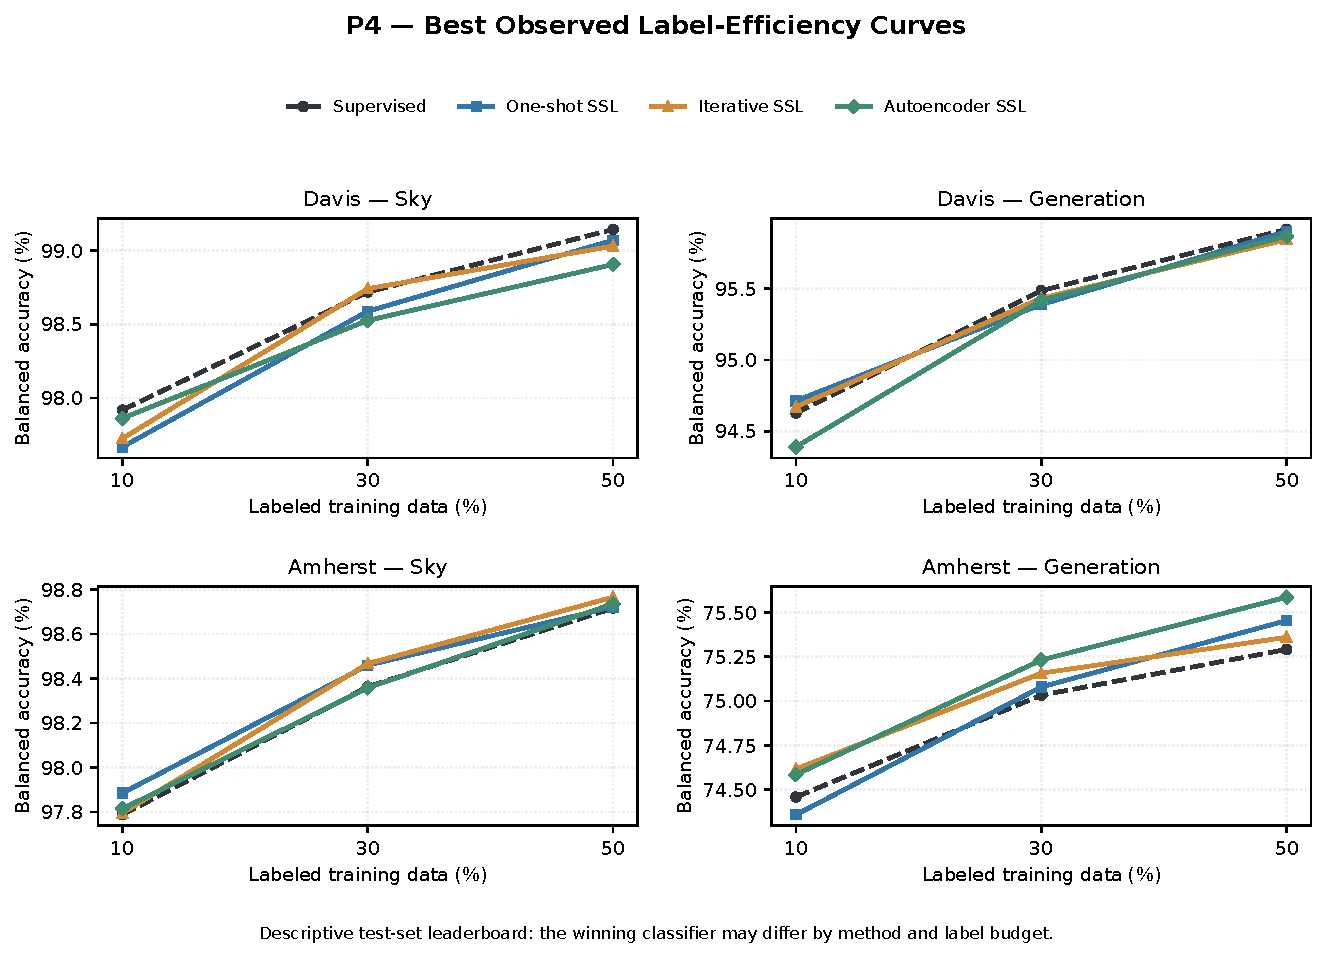
\includegraphics[width=\linewidth,height=5.62cm,keepaspectratio]{Figures/P4/P4_Best_Observed_Label_Efficiency_Overview.pdf}
\end{column}
\begin{column}{0.27\textwidth}
\factbox{Reading the curves}{x: labeled fraction. y: balanced accuracy.}\vspace{0.15cm}
\small \textbf{Each curve is a strategy, not a fixed classifier.} At every point the best observed result among Logistic, SVM, RF, XGBoost and MLP is shown. The winning classifier can change with label fraction.
\end{column}
\end{columns}
\footeridea{Unlike the preceding XGBoost tables, these curves select the best classifier anew at each point.}
\note{These are best-of-five-classifiers curves, not fixed-XGBoost curves. More labels help, but notice the
y-axis scale: the strategies are within a fraction of a point of each other, and even the
supervised model only loses about one point between 50 and 10 percent labels.}
\end{frame}

\begin{frame}{P4 — Can SSL beat supervised at 10\% labels?}
\sectiontag{P4 \quad RESULTS — THE QUESTION ASKED}
{\fontsize{8.4}{9.9}\selectfont
\setlength{\tabcolsep}{3.0pt}
\renewcommand{\arraystretch}{1.35}
\begin{tabular}{@{}llrlrlrr@{}}\toprule
\textbf{City} & \textbf{Task} & \multicolumn{2}{c}{\textbf{Best supervised}} & \multicolumn{2}{c}{\textbf{Best SSL}} & \shortstack{\textbf{Best-vs-best}\\\textbf{gain}} & \shortstack{\textbf{Largest same-model}\\\textbf{SSL improvement}}\\\midrule
Davis & Sky & 97.92 & XGB & 97.86 & XGB+AE & \textcolor{warn}{$-0.06$} & $+1.03$ (MLP+Iter.)\\
Davis & Generation & 94.63 & XGB & 94.71 & XGB+One-shot & $+0.08$ & \cellcolor{softteal}$\mathbf{+5.59}$ (MLP+AE)\\
Amherst & Sky & 97.79 & XGB & 97.88 & XGB+One-shot & $+0.09$ & $+0.54$ (MLP+Iter.)\\
Amherst & Generation & 74.46 & RF & 74.62 & RF+Iter. & $+0.16$ & $+0.36$ (LR+AE)\\
\bottomrule\end{tabular}}
\vspace{0.10cm}
\begin{columns}[T,totalwidth=\textwidth]
\begin{column}{0.48\textwidth}
\factbox{Answer: yes, marginally}{3 of 4 tasks, by 0.08--0.16 points --- below most seed SDs.}
\end{column}
\begin{column}{0.48\textwidth}
\factbox{Biggest win: the MLP}{AE SSL lifts the MLP 85.55 $\to$ 91.14\% on Davis generation (gain SD 8.80).}
\end{column}
\end{columns}
\smallmuted{Best-vs-best gain = best SSL BA minus best supervised BA (models may differ). Same-classifier improvement compares SSL to the supervised version of that \emph{same} model.}\par\vspace{0.08cm}
\note{This slide answers the exact question in the assignment. At ten percent labels, the best SSL
configuration beats the best supervised one in three of four tasks, but only by about a tenth of a
point. The largest same-classifier gain is for the MLP: autoencoder features raise it by 5.6 points on Davis
generation, though with a large spread across seeds.}
\end{frame}



\section{P5: Transfer Learning}

\begin{frame}{Problem 5 — Transfer Learning}
\sectiontag{P5 \quad PROBLEM}
\begin{block}{Objective from the assignment}
Use a \textbf{data-rich source city} to help a \textbf{data-poor target city}, and beat both baselines.
\end{block}
\vspace{0.05cm}
\begin{columns}[T,totalwidth=\textwidth]
\begin{column}{0.49\textwidth}
\begin{block}{SOURCE: Davis (6 years)}
\small \textbf{Zero-shot baseline:} train on Davis, predict Amherst directly.
\end{block}
\end{column}
\begin{column}{0.49\textwidth}
\begin{block}{TARGET: Amherst (3 years)}
\small $k=10,50,100$ labels. \textbf{Few-shot baseline:} train only on these.
\end{block}
\end{column}
\end{columns}
\vspace{0.12cm}
\begin{block}{Deliverable in the question}
\small Zero-shot, few-shot and transfer RMSE on one Amherst test set; discuss what transferred and what did not.
\end{block}
\note{Problem 5 brings everything together. Davis has six years of data; Amherst gets only 10, 50
or 100 labeled samples. There are two baselines to beat: zero-shot, which uses the Davis model
directly, and few-shot, which trains only on the Amherst labels.}
\end{frame}

\begin{frame}{P5 — Models and transfer strategies}
\sectiontag{P5 \quad MODELS}
\smallmuted{Source: Davis; target: Amherst; budgets: 10, 50, 100 target labels.}\vspace{0.20cm}
\renewcommand{\arraystretch}{1.30}
{\small
\begin{tabularx}{\linewidth}{@{}P{2.42cm}Y@{}}\toprule
\textbf{Family} & \textbf{Methods compared}\\\midrule
\rowcolor{softblue} Classical ML & Ridge, random forest, XGBoost (source-only and target-only baselines)\\
\rowcolor{softblue} Classical transfer & Affine calibration; joint calibrated source--target pooling\\
\rowcolor{softteal} Deep learning & PyTorch MLP\\
\rowcolor{softteal} Neural transfer & Frozen MLP encoder + Ridge head; partial fine-tuning\\\bottomrule
\end{tabularx}\par}
\vspace{0.15cm}
\smallmuted{Classical methods correct outputs or data; neural methods reuse features or selected network weights.}
\note{There are four transfer strategies: two classical ones, affine calibration and joint
pooling, and two neural ones, a frozen encoder with a new Ridge head, and partial fine-tuning.}
\end{frame}

\begin{frame}{P5 — Transfer methods in plain language}
\sectiontag{P5 \quad METHODS — HOW SOURCE KNOWLEDGE IS REUSED}
{\small\renewcommand{\arraystretch}{1.25}
\begin{tabularx}{\linewidth}{@{}P{3.25cm}Y@{}}\toprule
\textbf{Strategy} & \textbf{What the model actually does}\\\midrule
Affine calibration & Fits a scale and offset to correct Davis-model predictions using the small labeled Amherst set.\\
Joint calibrated pooling & Calibrates source information and combines it with Amherst's few labeled examples to train a joint regressor.\\
Frozen encoder $+$ Ridge & Keeps the source-trained neural feature extractor fixed; fits a new ridge regression head on Amherst labels.\\
Partial fine-tuning & Reuses pretrained neural weights but updates selected layers with Amherst examples.\\
\bottomrule\end{tabularx}}
\vspace{0.18cm}
\begin{block}{Why compare these?}
\footnotesize They range from a simple output correction to neural representation adaptation. The key test is whether each beats \emph{both} source-only zero-shot and matched target-only few-shot baselines.
\end{block}
\note{Affine calibration learns two correction parameters: scale and offset. Joint pooling uses the adjusted source data together with the small target set. Frozen-encoder transfer fits a new Ridge predictor on source-trained neural features. Partial fine-tuning lets some of the neural layers adapt. The fair baseline is to train using the same Amherst labels without Davis information.}
\end{frame}

\begin{frame}{P5 — All strategies: best base model for each method}
\sectiontag{P5 \quad RESULTS — COMPARE ALL METHODS}
\smallmuted{Amherst test RMSE (kW), three-seed mean; lower is better. The base regressor may change by strategy and label budget: each cell reports that method's best observed base model.}
\vspace{0.16cm}
{\footnotesize
\setlength{\tabcolsep}{7.0pt}
\renewcommand{\arraystretch}{1.47}
\centering
\begin{tabular}{@{}lrrr@{}}\toprule
\textbf{Strategy} & \textbf{10 labels} & \textbf{50 labels} & \textbf{100 labels}\\\midrule
Source-only zero-shot & 75.82 (Ridge) & 75.82 (Ridge) & 75.82 (Ridge)\\
Target-only few-shot & 26.19 (Ridge) & \textcolor{teal}{\textbf{22.03 (Ridge)}} & 22.04 (RF)\\
Affine calibration & 24.30 (XGB) & 22.68 (XGB) & 22.60 (XGB)\\
Joint calibrated pooling & \textcolor{teal}{\textbf{23.22 (Ridge)}} & 22.03 (Ridge) & \textcolor{teal}{\textbf{21.80 (RF)}}\\
Frozen encoder + Ridge & 27.12 (MLP) & 25.64 (MLP) & 24.20 (MLP)\\
Partial fine-tuning & 24.33 (MLP) & 23.03 (MLP) & 22.21 (MLP)\\
\bottomrule\end{tabular}\par}
\vspace{0.20cm}
\smallmuted{The source-only model uses no Amherst labels, so its RMSE is constant across the three columns. Teal values highlight the lowest observed RMSE for each label budget.}
\footeridea{Pooling is strongest with 10 and 100 labels; a target-only model is just as good at 50.}
\note{This table demonstrates that all six strategies were evaluated. Zero-shot fails badly. With ten labels, classical joint calibrated pooling and Ridge has the best error. At fifty labels it ties the target-only Ridge result. At one hundred labels, pooled random forest has the lowest error. Frozen-feature and partially fine-tuned neural transfer were also tested and did not win.}
\end{frame}

\begin{frame}{P5 — Controlled test: fix the base regressor}
\sectiontag{P5 \quad RESULTS — TARGET-ONLY VS ADAPTED, SAME MODEL}
\smallmuted{For each row, hold the base regressor, Amherst label budget, split, and seeds fixed. Only use of Davis source knowledge changes. Positive gain = lower RMSE with transfer.}
\vspace{0.17cm}
{\footnotesize\setlength{\tabcolsep}{8pt}\renewcommand{\arraystretch}{1.44}
\begin{tabular}{@{}llrrr@{}}\toprule
\textbf{Fixed base regressor} & \textbf{Transfer strategy} & \textbf{10 labels} & \textbf{50 labels} & \textbf{100 labels}\\\midrule
Ridge & Joint pooling & \textcolor{teal}{\textbf{+2.97}} & +0.00 & +0.28\\
Random forest & Joint pooling & \textcolor{teal}{\textbf{+5.48}} & +0.40 & +0.24\\
XGBoost & Joint pooling & \textcolor{teal}{\textbf{+6.28}} & +2.30 & +0.78\\
MLP & Partial fine-tuning & \textcolor{teal}{\textbf{+4.98}} & +0.91 & +2.03\\
\bottomrule\end{tabular}}
\vspace{0.20cm}
\begin{block}{How to read the gains}
\footnotesize Each gain (kW) is \textbf{target-only RMSE minus adapted RMSE} for the \emph{same base model}. For example, Ridge at 10 labels: $26.19 - 23.22 = 2.97$ kW. Some other adaptations (such as affine calibration) have \emph{negative} gains; see the full report.
\end{block}
\note{This is a controlled transfer comparison. We compare the exact same base-model family with and without source-city knowledge, using identical target-label budgets. Ridge at ten labels improves by 2.97 kilowatts, while XGBoost joint pooling improves over its own target-only baseline by 6.28 kilowatts. These are matched same-model gains, not the best-of-all-method leaderboard shown next.}
\end{frame}

\begin{frame}{P5 — Summary: zero-shot, few-shot, and best transfer}
\sectiontag{P5 \quad BEST OBSERVED — AFTER ALL STRATEGIES}
{\small\centering\begin{tabular}{@{}rllll@{}}\toprule
\textbf{$k$} & \textbf{Zero-shot} & \textbf{Target-only} & \textbf{Best transfer} & \shortstack{\textbf{Gain vs}\\\textbf{target-only}}\\\midrule
\rowcolor{softteal} 10 & 75.82 (Ridge) & 26.19 (Ridge) & \textbf{23.22} (pooling, Ridge) & \textbf{+2.97}\\
50 & 75.82 (Ridge) & \textbf{22.03} (Ridge) & 22.03 (pooling, Ridge) & +0.00\\
100 & 75.82 (Ridge) & 22.04 (RF) & \textbf{21.80} (pooling, RF) & +0.24\\\bottomrule
\end{tabular}\par}\vspace{0.20cm}
\begin{columns}[T,totalwidth=\textwidth]
\begin{column}{0.49\textwidth}
\factbox{Both baselines beaten at $k=10$}{$-69\%$ vs zero-shot and $-11\%$ vs ten-label target-only.}
\end{column}
\begin{column}{0.49\textwidth}
\factbox{Diminishing returns}{As $k$ grows, the target-only model catches up and the transfer advantage shrinks.}
\end{column}
\end{columns}
\footeridea{RMSE (kW), three-seed mean. Gain = target-only RMSE $-$ transfer RMSE at the same $k$; values are best-observed strategies, not a fixed-model comparison.}
\note{This is the comparison the assignment asks for. With ten labels, pooling beats zero-shot by
69 percent and the target-only model by 11 percent, so it beats both baselines. With more labels the
target-only model catches up and the advantage shrinks.}
\end{frame}

\begin{frame}{P5 — What transferred and what did not}
\sectiontag{P5 \quad ANALYSIS}
\begin{columns}[T,totalwidth=\textwidth]
\begin{column}{0.49\textwidth}
\begin{block}{Transferred: the \emph{shape}}
\small How irradiance, zenith angle and temperature drive power. Target-based calibration can correct part of the raw-kW prediction bias.
\end{block}
\end{column}
\begin{column}{0.49\textwidth}
\begin{block}{Did not transfer: the \emph{scale}}
\small Installed capacity and site-specific effects (snow, soiling, downtime). Target labels help correct the output scale.
\end{block}
\end{column}
\end{columns}
\vspace{0.2cm}

\note{So what transferred? Some feature relationships are reusable; target labels help adjust the output scale. What did not transfer is the absolute scale and site-specific
effects, which can only be examined using target observations. The result suggests that adapting a source model with limited target data can be more useful than applying it unchanged.}
\end{frame}



\section{Conclusions}





\begin{frame}{Final finding — ten target labels transform cross-city prediction}
\sectiontag{MAIN RESULT — DAVIS $\rightarrow$ AMHERST}
\begin{columns}[T,totalwidth=\textwidth]
\begin{column}{0.50\textwidth}
\centering
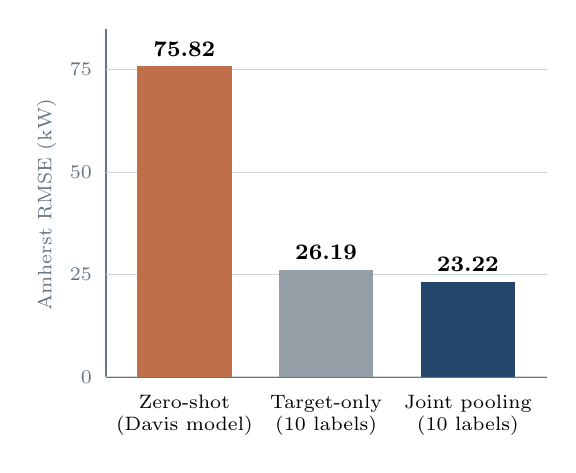
\begin{tikzpicture}[x=1cm,y=0.052cm]
  \draw[slate,line width=0.8pt] (0,0) -- (5.6,0);
  \draw[slate,line width=0.8pt] (0,0) -- (0,85);
  \foreach \v in {0,25,50,75}{\draw[slate!30] (0,\v) -- (5.6,\v); \node[font=\scriptsize,text=slate,anchor=east] at (-0.05,\v) {\v};}
  \fill[warn!85] (0.4,0) rectangle (1.6,75.82); \node[font=\footnotesize\bfseries,above] at (1.0,75.82) {75.82};
  \fill[slate!70] (2.2,0) rectangle (3.4,26.19); \node[font=\footnotesize\bfseries,above] at (2.8,26.19) {26.19};
  \fill[navy] (4.0,0) rectangle (5.2,23.22); \node[font=\footnotesize\bfseries,above] at (4.6,23.22) {23.22};
  \node[font=\scriptsize,align=center,anchor=north] at (1.0,-2) {Zero-shot\\(Davis model)};
  \node[font=\scriptsize,align=center,anchor=north] at (2.8,-2) {Target-only\\(10 labels)};
  \node[font=\scriptsize,align=center,anchor=north] at (4.6,-2) {Joint pooling\\(10 labels)};
  \node[font=\scriptsize,text=slate,rotate=90] at (-0.75,42) {Amherst RMSE (kW)};
\end{tikzpicture}
\end{column}
\begin{column}{0.47\textwidth}
\small
\begin{itemize}\setlength\itemsep{0.4em}
\item At home, Davis models reach $\approx$5\% nRMSE; elsewhere they exceed \textbf{100\%}.
\item A large \textbf{power-scale mismatch} contributes to poor zero-shot transfer.
\item \textbf{Ten} target labels re-anchor the scale: \textbf{$-69\%$} RMSE vs zero-shot, $-11\%$ vs target-only.
\end{itemize}
\end{column}
\end{columns}
\footeridea{With 10 target labels, joint calibrated pooling outperforms both the zero-shot and matched target-only baselines.}
\note{The most important result is this cross-city comparison. Applied unchanged to Amherst, the source-only Davis model gives 75.82 kilowatts RMSE. With ten labeled Amherst observations, the target-only Ridge baseline reaches 26.19 kilowatts; joint calibrated pooling reaches 23.22 kilowatts. That is 69 percent lower error than zero-shot, and 2.97 kilowatts better than the matched target-only baseline. Different site power scales are an important part of why direct transfer is difficult.}
\end{frame}

% -------------------------------------------------------------
% -------------------------------------------------------------
% Final slide: standard Madrid title bar and footer
% -------------------------------------------------------------
\begin{frame}{Closing}
\sectiontag{THANK YOU}
\vfill
\begin{center}
{\Huge\bfseries\color{navy}Thank You!}\\[0.45cm]
{\LARGE\color{teal}Have a Great Day!}
\end{center}
\vfill
\begin{center}\small
\textbf{Video presentation:}\\[1pt]
{\footnotesize\href{\videourl}{\nolinkurl{\videourl}}}\\[4pt]
\textbf{Code, results and report:}\\[1pt]
{\footnotesize\href{\repourl}{\nolinkurl{\repourl}}}
\end{center}
\note{Thank you for watching, and have a great day!}
\end{frame}

\ifshowbackup
\appendix
\section{Supplementary Results (Optional Backup Slides)}
% Supplementary slides omitted from the main recording.
\begin{frame}{Roadmap: five learning problems}
\sectiontag{PROJECT SCOPE}
\vspace{-0.12cm}
\begin{columns}[T,totalwidth=\textwidth]
\begin{column}{0.485\textwidth}
\begin{block}{P1 — Classification}Can weather measurements identify sky conditions and power-generation regimes?\end{block}
\begin{block}{P2 — Regression}How accurately can PV power be estimated, including in unseen cities?\end{block}
\begin{block}{P3 — Dimensionality Reduction}Can 2, 5, or 10 latent features replace the full input vector?\end{block}
\end{column}
\begin{column}{0.485\textwidth}
\begin{block}{P4 — Semi-Supervised Learning}Can unlabeled data help when only 10--50\% of training labels are available?\end{block}
\begin{block}{P5 — Transfer Learning}Can a data-rich source city help predict power in a label-scarce target city?\end{block}
\vspace{0.15cm}
\begin{beamercolorbox}[rounded=true,sep=0.20cm]{block body}
\textbf{One common principle:} chronological evaluation, train-only preprocessing and matched baselines.
\end{beamercolorbox}
\end{column}
\end{columns}
\note{The project has five problems, one per learning paradigm. P1 is classification, P2 is
regression, P3 is dimensionality reduction, P4 is semi-supervised learning, and P5 is transfer
learning between cities. All five share one rule: split by time, fit preprocessing on training
data only, and always compare against a fair baseline.}
\end{frame}

% Moved P2 — Three vs six years of history into main presentation.


\begin{frame}{Limitations, reproducibility and next steps}
\sectiontag{FINAL TAKEAWAYS}
\begin{columns}[T,totalwidth=\textwidth]
\begin{column}{0.32\textwidth}
\begin{block}{Limitations}
\scriptsize\begin{itemize}
\setlength\itemsep{0.08em}
\item Five sites; different capacities.
\item Three seeds; best-test scores are descriptive.
\item Sky labels have irradiance proxies ($\approx$99.8\% proxy check).
\item Zero-shot without per-city target normalization.
\end{itemize}
\end{block}
\end{column}
\begin{column}{0.32\textwidth}
\begin{block}{Reproducibility}
\scriptsize\begin{itemize}
\setlength\itemsep{0.08em}
\item Seeds 42, 123, 2026.
\item Chronological splits; saved indices.
\item Train-only preprocessing.
\item Code, README, requirements and results files in the repository.
\end{itemize}
\end{block}
\end{column}
\begin{column}{0.32\textwidth}
\begin{block}{Next steps}
\scriptsize\begin{itemize}
\setlength\itemsep{0.08em}
\item GRU / TCN for sequences.
\item Per-city normalized target.
\item Feature-level domain adaptation.
\item Supervised reducers.
\end{itemize}
\end{block}
\end{column}
\end{columns}
\vspace{0.15cm}
\begin{beamercolorbox}[sep=0.13cm,wd=\linewidth]{block body}
\small\textbf{Bottom line:} learn the weather-to-power shape from data-rich sites, then re-anchor the scale with a handful of local labels.
\end{beamercolorbox}
\note{Some limitations: only five sites, three seeds, and the sky labels can be partly reconstructed
from other irradiance columns. My zero-shot test also skipped per-city target normalization, which
is the first thing I'd add. Everything is reproducible with fixed seeds and saved splits. Next steps
are a GRU, normalized targets, and proper domain adaptation.}
\end{frame}

\begin{frame}{Headline results at a glance}
\sectiontag{PREVIEW}
{\footnotesize
\renewcommand{\arraystretch}{1.28}
\setlength{\tabcolsep}{4pt}
\begin{tabularx}{\linewidth}{@{}P{0.6cm}P{4.2cm}YP{3.3cm}@{}}\toprule
 & \textbf{Setting} & \textbf{Best result (model)} & \textbf{Reference}\\\midrule
P1 & Sky condition, Davis / Amherst & \textbf{99.15\%} / 98.82\% BA (XGBoost) & chance = 33.3\%\\
P1 & Generation regime, Davis / Amherst & 96.35\% (XGBoost) / \textcolor{warn}{\textbf{75.90\%}} (RF) & Medium recall 60.8\%\\
P2 & Same-city RMSE, Davis / Amherst & \textbf{11.85\,kW} (4.72\%) / 19.96\,kW (15.69\%) & Ridge 13.82 / 20.72\\
P2 & Zero-shot Davis $\to$ 3 cities & 77--115\,kW RMSE, \textcolor{warn}{\textbf{$>$100\% nRMSE}} & in-city $\approx$6\%\\
P3 & Best compressed vs raw & raw features win \textbf{8 / 8} & closest: $-0.5$ BA pts\\
P4 & 10\% labels: best SSL vs best supervised & $+0.08$ to $+0.16$ BA pts (3 of 4) & MLP: $+5.59$ pts\\
\rowcolor{softteal} P5 & Davis $\to$ Amherst, 10 labels & \textbf{23.22\,kW} (joint pooling) & zero-shot 75.82\\
\bottomrule\end{tabularx}}
\footeridea{All values are held-out means over three seeds (42, 123, 2026).}
\note{Here is the whole story on one slide. Sky classification is almost perfect, but
generation regimes in Amherst are hard. Same-city regression is accurate, but models moved to a
new city fail badly. Compression never beat raw features, semi-supervised learning gives only tiny
gains, and transfer learning with just ten labels gives the biggest practical win. The rest of the
talk explains each line.}
\end{frame}

\begin{frame}{P1 — Results: sky and generation accuracy}
\sectiontag{P1 \quad RESULTS}
\vspace{0.05cm}
{\small\begin{tabular}{@{}llrr@{}}\toprule
\textbf{Task} & \textbf{Best observed model} & \textbf{Davis BA} & \textbf{Amherst BA}\\\midrule
Sky & XGBoost & \cellcolor{softteal}\textbf{99.15\%} & \cellcolor{softteal}\textbf{98.82\%}\\
Generation & XGBoost (Davis); RF (Amherst) & \cellcolor{softteal}\textbf{96.35\%} & \cellcolor{softteal}\textbf{75.90\%}\\\bottomrule
\end{tabular}}\par\vspace{0.28cm}
\begin{columns}[T,totalwidth=\textwidth]
\begin{column}{0.48\textwidth}
\factbox{Sky tasks}{Very high balanced accuracy in both cities; remaining irradiance columns (DHI, DNI) carry much of the label signal.}
\end{column}
\begin{column}{0.48\textwidth}
\factbox{Generation tasks}{Davis is much easier than Amherst: about 20 points apart.}
\end{column}
\end{columns}
\footeridea{High sky scores describe nowcasting from simultaneous measurements, not forecasting tomorrow's sky.}
\note{Sky classification reaches 99.15 percent balanced accuracy in Davis and 98.82 in Amherst,
both with XGBoost. Generation regimes are a different story: 96 percent in Davis but only about 76
percent in Amherst. Keep that 20-point gap in mind; it comes back in P2 and P5.}
\end{frame}

% Moved P1 — Amherst sky confusion matrices into main presentation.


% Moved P1 — Davis generation confusion matrices into main presentation.


\begin{frame}{P1 — Per-class recall: which class is hardest?}
\sectiontag{P1 \quad RESULTS — PER-CLASS RECALL}
\smallmuted{Recall (\%): diagonal of the row-normalized confusion matrices; means over three seeds.}
\vspace{0.13cm}
{\small
\setlength{\tabcolsep}{7pt}
\renewcommand{\arraystretch}{1.48}
\begin{tabular}{@{}llrrrr@{}}\toprule
\textbf{City} & \textbf{Task} & \textbf{Class 1} & \textbf{Class 2} & \textbf{Class 3} & \textbf{Model}\\\midrule
Davis & Sky & 99.6 & \cellcolor{softgold}\textbf{98.1} & 99.7 & XGBoost\\
Amherst & Sky & 99.8 & \cellcolor{softgold}\textbf{97.4} & 99.3 & XGBoost\\
Davis & Generation & 96.8 & \cellcolor{softgold}\textbf{93.6} & 98.7 & XGBoost\\
Amherst & Generation & 76.5 & \cellcolor{softgold}\textbf{60.8} & 90.4 & Random forest\\
\bottomrule\end{tabular}}\par\vspace{0.16cm}
\begin{block}{Class definitions}
\footnotesize Sky: 1 = Overcast; 2 = Partly Cloudy; 3 = Clear. \quad
Generation: 1 = Low; 2 = Medium; 3 = High. \textbf{Shaded = lowest recall in each row.}
\end{block}
\footeridea{The middle class is always the hardest; Amherst Medium is the worst at 60.8\%.}
\note{Putting the four best models side by side: in every row the hardest class is the middle one,
Partly Cloudy or Medium. Amherst Medium is by far the worst, at 60.8 percent recall.}
\end{frame}

\begin{frame}{P2 — Results: Davis same-city}
\sectiontag{P2 \quad RESULTS — SAME-CITY DAVIS}
\small
\begin{tabularx}{\linewidth}{@{}P{3.15cm}YYY@{}}\toprule
\textbf{Model} & \textbf{RMSE (kW)} & \textbf{MAE (kW)} & \textbf{nRMSE (\%)} \\\midrule
Ridge & 13.82 $\pm$ 0.00 & 8.49 $\pm$ 0.00 & 5.50 $\pm$ 0.00 \\
RBF SVR & 14.14 $\pm$ 0.00 & 10.03 $\pm$ 0.00 & 5.63 $\pm$ 0.00 \\
Random forest & 11.95 $\pm$ 0.01 & \textbf{5.75 $\pm$ 0.01} & 4.76 $\pm$ 0.01 \\
\rowcolor{softteal}\textbf{XGBoost} & \textbf{11.85 $\pm$ 0.08} & 6.33 $\pm$ 0.03 & \textbf{4.72 $\pm$ 0.03} \\
MLP (PyTorch) & \textbf{11.85 $\pm$ 0.27} & 6.52 $\pm$ 0.44 & \textbf{4.72 $\pm$ 0.11} \\
\bottomrule\end{tabularx}\par
\vspace{0.25cm}
\begin{block}{Reading the table}
\footnotesize XGBoost and the MLP tie at 11.85\,kW (XGBoost has lower seed variance). Trees cut Ridge's error by about 14\%. Lower is better.
\end{block}
\note{In Davis, XGBoost and the MLP tie at 11.85 kilowatts RMSE, which is 4.7 percent of the
power range. Tree models cut the linear Ridge error by about 14 percent, because power depends on
irradiance in a non-linear way with interactions.}
\end{frame}

\begin{frame}{P2 — Results: Amherst same-city}
\sectiontag{P2 \quad RESULTS — SAME-CITY AMHERST}
\small
\begin{tabularx}{\linewidth}{@{}P{3.15cm}YYY@{}}\toprule
\textbf{Model} & \textbf{RMSE (kW)} & \textbf{MAE (kW)} & \textbf{nRMSE (\%)} \\\midrule
Ridge & 20.72 $\pm$ 0.00 & 14.61 $\pm$ 0.00 & 16.29 $\pm$ 0.00 \\
RBF SVR & 25.79 $\pm$ 0.00 & 19.52 $\pm$ 0.00 & 20.28 $\pm$ 0.00 \\
Random forest & 20.17 $\pm$ 0.04 & \textbf{13.58 $\pm$ 0.02} & 15.86 $\pm$ 0.03 \\
XGBoost & 20.12 $\pm$ 0.21 & 13.78 $\pm$ 0.18 & 15.82 $\pm$ 0.17 \\
\rowcolor{softteal}\textbf{MLP (PyTorch)} & \textbf{19.96 $\pm$ 0.05} & 14.09 $\pm$ 0.14 & \textbf{15.69 $\pm$ 0.04} \\
\bottomrule\end{tabularx}\par
\vspace{0.25cm}
\begin{block}{Reading the table}
\footnotesize Amherst error is about 3$\times$ Davis in nRMSE (15.7\% vs 4.7\%), consistent with the hard Amherst generation classes in P1.
\end{block}
\note{In Amherst the MLP is best at about 20 kilowatts, but in normalized terms the error is more
than three times the Davis error. That matches what we saw in P1: Amherst weather explains its power
much less well.}
\end{frame}

\begin{frame}{P2 — Results: sequential forecasting ($K=12$)}
\sectiontag{P2 \quad RESULTS — NEXT-STEP FORECAST}
\small
\begin{tabularx}{\linewidth}{@{}P{3.0cm}YYYY@{}}\toprule
\textbf{Model} & \textbf{Davis RMSE} & \textbf{Davis nRMSE} & \textbf{Amherst RMSE} & \textbf{Amherst nRMSE}\\\midrule
Ridge & 13.58 & 5.40 & 17.12 & 13.46\\
RBF SVR & 18.48 & 7.36 & 20.41 & 16.04\\
\rowcolor{softteal}\textbf{Random forest} & \textbf{13.30} & \textbf{5.29} & \textbf{15.96} & \textbf{12.54}\\
XGBoost & 13.49 & 5.37 & 16.06 & 12.62\\
LSTM (PyTorch) & 14.64 & 5.83 & 16.55 & 13.01\\
\bottomrule\end{tabularx}\par
\vspace{0.2cm}
\begin{columns}[T,totalwidth=\textwidth]
\begin{column}{0.48\textwidth}
\factbox{LSTM does not win}{With a short 12-step window, trees over flattened lags are as expressive and more stable.}
\end{column}
\begin{column}{0.48\textwidth}
\factbox{History helps Amherst}{Amherst: 15.96\,kW sequential vs 19.96\,kW same-city. Recent output carries site effects the weather lacks.}
\end{column}
\end{columns}
\smallmuted{RMSE in kW, nRMSE in \%, means over three seeds. Sequential and same-city use different inputs, so the comparison is indicative.}
\note{For next-step forecasting, random forest wins in both cities and the LSTM is not better. An
interesting detail: in Amherst the sequential model beats the same-city model, while in Davis it is
the other way round. Where weather explains power poorly, recent power readings add information.}
\end{frame}

\begin{frame}{P2 — Zero-shot: all models (RMSE, kW)}
\sectiontag{P2 \quad RESULTS — ZERO-SHOT TABLE}
\small
\begin{tabularx}{\linewidth}{@{}P{3.0cm}YYYY@{}}\toprule
\textbf{Model} & \textbf{Davis (ID)} & \textbf{Huron} & \textbf{La Jolla} & \textbf{Santa Barbara}\\\midrule
Ridge & 16.95 & 124.95 & 130.18 & 126.01\\
\rowcolor{softteal}\textbf{RBF SVR} & 16.32 & \textbf{114.61} & \textbf{77.27} & \textbf{102.96}\\
Random forest & 15.21 & 124.49 & 124.75 & 125.03\\
XGBoost & \textbf{14.88} & 125.72 & 121.48 & 121.11\\
MLP (PyTorch) & 15.19 & 123.57 & 123.47 & 120.76\\
\bottomrule\end{tabularx}\par
\vspace{0.22cm}
\begin{block}{Why is SVR the ``least bad''?}
\footnotesize Likely because an RBF model relaxes towards its bias term far from the training data, so it extrapolates the Davis scale less. Its advantage is largest at La Jolla (112.7\% vs 177--190\% nRMSE). Best-model MAE: 107.38 / 75.88 / 98.68\,kW.
\end{block}
\note{Here are the numbers. The best in-city model, XGBoost, is one of the worst out of city. The
RBF SVR is the least bad everywhere, probably because a kernel model falls back towards its bias
far from the training data, so it extrapolates the Davis scale less. But even SVR is far from usable.}
\end{frame}

\begin{frame}{P3 — Preprocessing and train-only fitting}
\sectiontag{P3 \quad PREPROCESSING}
\begin{enumerate}\setlength\itemsep{0.38em}
\item Use the \textbf{same chronological indices} and feature exclusions as P1/P2.
\item Fit the scaler and encoder \textbf{only on training inputs}.
\item Fit PCA / Kernel PCA / Autoencoder \textbf{without labels} on training data.
\item Transform training and test sets into 2, 5 or 10 dimensions.
\item Train the downstream model on training embeddings; score on test embeddings.
\end{enumerate}
\vspace{0.08cm}
\factbox{Raw-feature reference}{Every compressed configuration is compared with the same model on the original preprocessed features.}
\note{The procedure: same splits as before, fit the reducer on training inputs only, transform
both partitions, then train and test the downstream model. Each compressed result is compared with
the same model on the full features.}
\end{frame}

\begin{frame}{P3 — How was $d$ chosen?}
\sectiontag{P3 \quad ANALYSIS — ELBOW}
\begin{columns}[T,totalwidth=\textwidth]
\begin{column}{0.46\textwidth}
{\small\renewcommand{\arraystretch}{1.3}
\begin{tabular}{@{}lrrr@{}}\toprule
\textbf{PCA variance (\%)} & $d{=}2$ & $d{=}5$ & $d{=}10$\\\midrule
Davis Sky & 34.3 & 63.7 & 84.4\\
Davis Regression & 36.9 & 65.2 & 85.1\\
Amherst Sky & 39.9 & 65.9 & 85.5\\
Amherst Regression & 41.9 & 67.2 & 86.4\\
\bottomrule\end{tabular}}
\end{column}
\begin{column}{0.50\textwidth}
\begin{itemize}\setlength\itemsep{0.35em}\small
\item \textbf{Knee at $d=5$:} components 3--5 add $\approx$9.8 points each; 6--10 only $\approx$4.2 each.
\item No $d\le10$ reaches 90\% variance.
\item \textbf{Downstream confirms $d=10$:} best reduced score in 7 of 8 settings ($d=5$ only for Davis generation).
\end{itemize}
\end{column}
\end{columns}
\vspace{0.2cm}
\factbox{Choice}{Operate at $d=10$; $d=5$ is the knee of the variance curve.}
\note{How should d be chosen? The variance curve bends around five components: after that each
extra component adds less than half as much. But downstream accuracy keeps improving, and d equals
10 gives the best compressed result in seven of eight settings, so I use 10 as the operating point.}
\end{frame}

\begin{frame}{P3 — Classification after compression}
\sectiontag{P3 \quad RESULTS — CLASSIFICATION}
\begin{columns}[T,totalwidth=\textwidth]
\begin{column}{0.67\textwidth}
\centering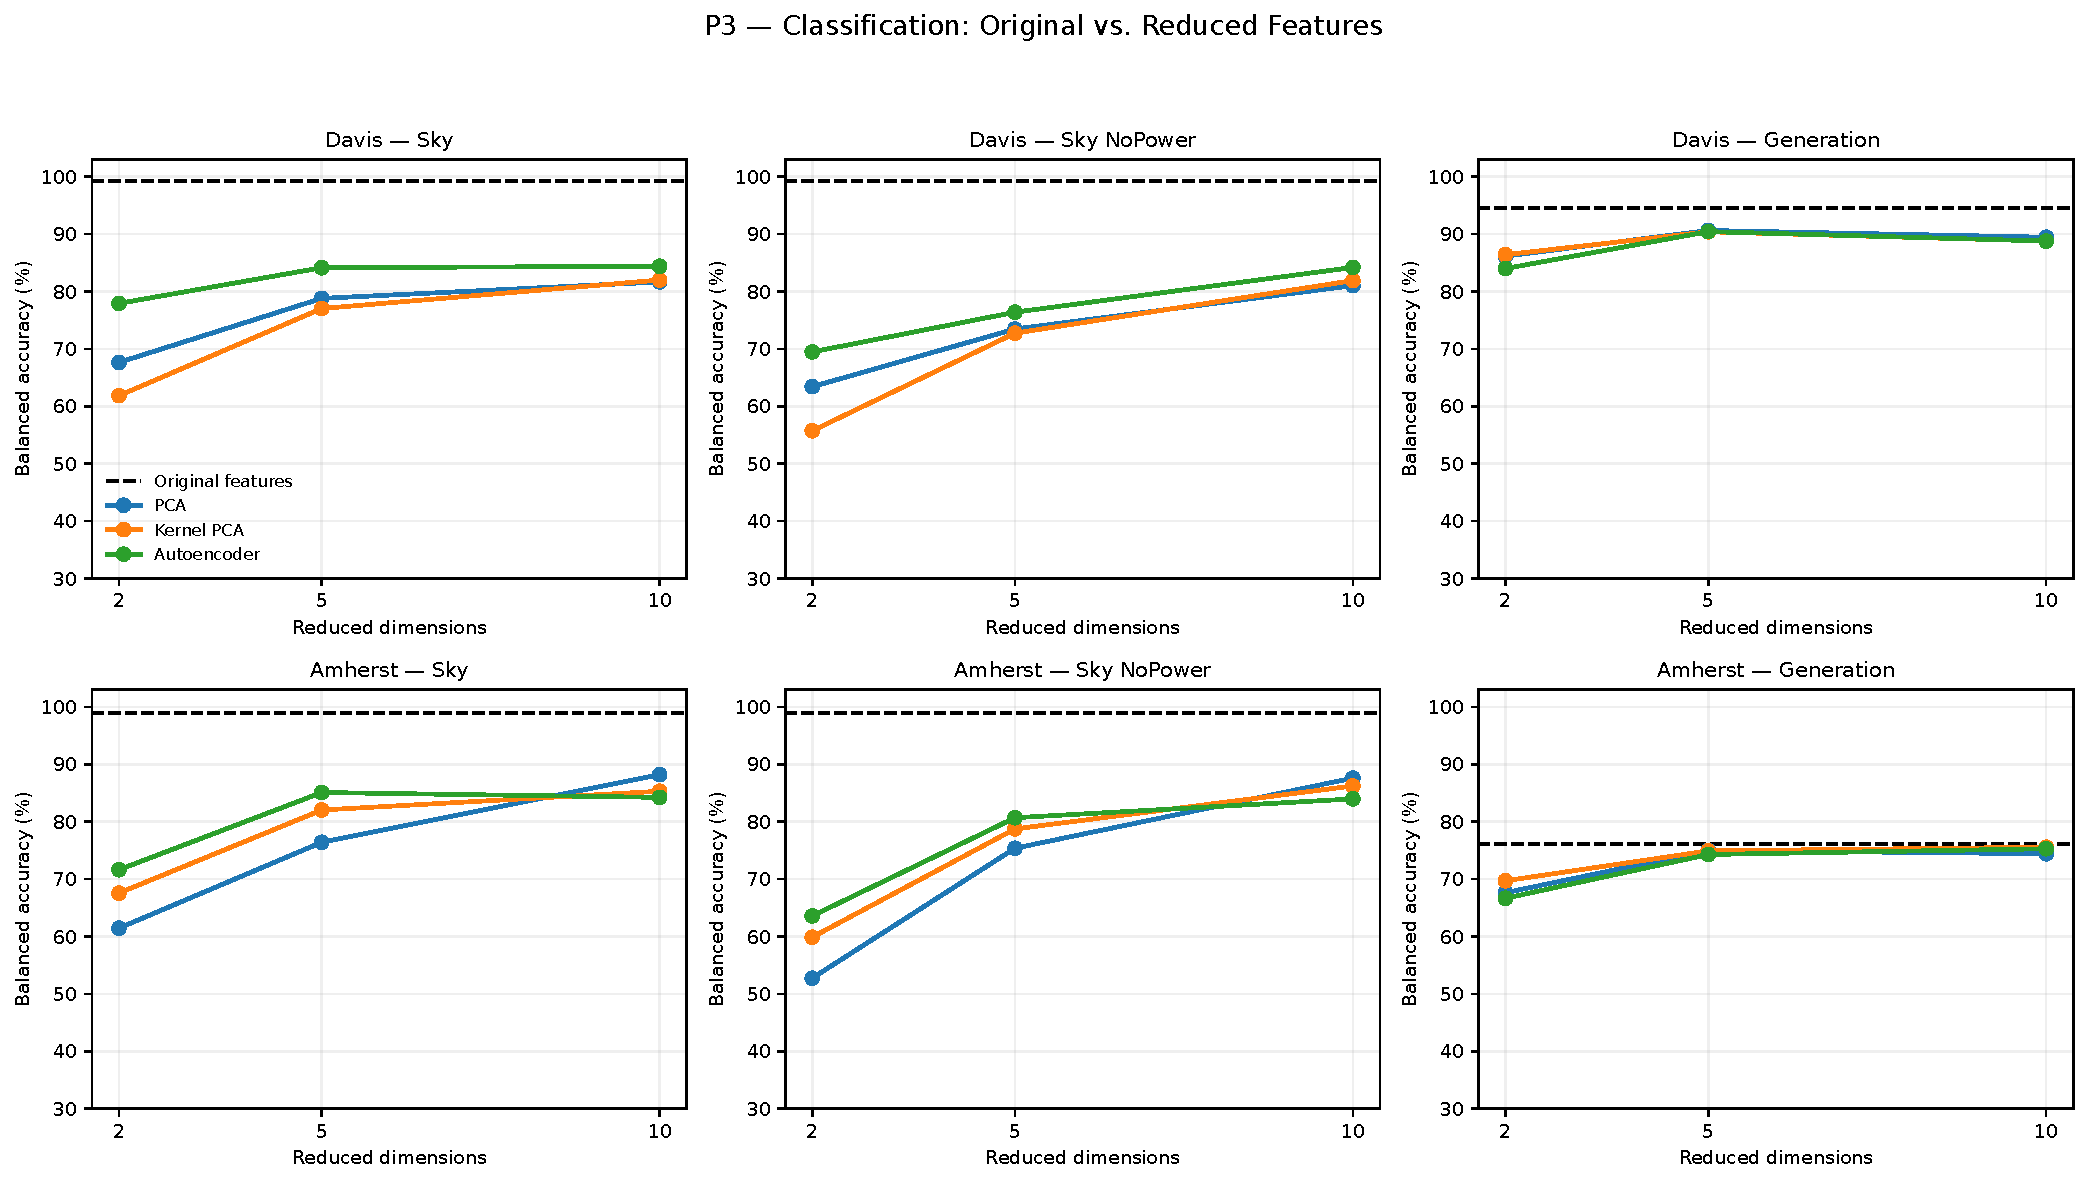
\includegraphics[width=\linewidth,height=5.6cm,keepaspectratio]{Figures/P3/P3_Classification_All_Methods.pdf}
\end{column}
\begin{column}{0.30\textwidth}
\factbox{Comparisons}{Original features (dashed) versus PCA, kernel PCA and autoencoder inputs.}\vspace{0.18cm}
\small \textbf{At $d=10$:} Davis Sky AE 84.40\% vs raw 99.17\%.\\[3pt]
\textbf{At $d=2$:} the autoencoder is the best reducer on every sky task.
\end{column}
\end{columns}
\footeridea{Compression reduces input size, but the full-input classifier stays stronger.}
\note{Here balanced accuracy is plotted against d, with the full-feature result as a dashed line.
Every curve stays below the line. The sky task suffers most: about 15 points lost in Davis even at
10 dimensions. At very small d, the non-linear autoencoder is the best reducer.}
\end{frame}

\begin{frame}{P3 — Downstream models: sky-condition classification}
\sectiontag{P3 \quad RESULTS — 10-DIMENSIONAL INPUTS}
\smallmuted{Balanced accuracy (\%), higher is better; mean over three seeds.}\vspace{0.18cm}
\begin{columns}[T,onlytextwidth]
\begin{column}{0.486\textwidth}
\textbf{Davis}\hfill{\scriptsize raw best: 99.17}\par\vspace{0.12cm}
{\fontsize{8.8}{10.4}\selectfont
\setlength{\tabcolsep}{3.9pt}
\renewcommand{\arraystretch}{1.39}
\begin{tabular}{@{}lrrr@{}}\toprule
\textbf{Model} & \textbf{PCA} & \textbf{KPCA} & \textbf{AE}\\\midrule
Logistic & 80.40 & 80.36 & 83.28\\
RBF SVM & 78.91 & 81.83 & \textcolor{teal}{\textbf{84.40}}\\
RF & 80.51 & 81.86 & 81.64\\
XGBoost & 81.09 & 81.23 & 82.69\\
MLP & 81.66 & 81.99 & 84.08\\
\bottomrule\end{tabular}}
\end{column}
\begin{column}{0.486\textwidth}
\textbf{Amherst}\hfill{\scriptsize raw best: 98.98}\par\vspace{0.12cm}
{\fontsize{8.8}{10.4}\selectfont
\setlength{\tabcolsep}{3.9pt}
\renewcommand{\arraystretch}{1.39}
\begin{tabular}{@{}lrrr@{}}\toprule
\textbf{Model} & \textbf{PCA} & \textbf{KPCA} & \textbf{AE}\\\midrule
Logistic & 86.64 & 84.03 & 81.95\\
RBF SVM & \textcolor{teal}{\textbf{88.19}} & 85.18 & 84.23\\
RF & 85.01 & 83.75 & 81.57\\
XGBoost & 86.27 & 84.04 & 81.22\\
MLP & 87.68 & 85.31 & 82.35\\
\bottomrule\end{tabular}}
\end{column}
\end{columns}
\vspace{0.30cm}
\begin{beamercolorbox}[wd=\linewidth,sep=0.14cm]{block body}
\footnotesize \textcolor{teal}{\textbf{Teal}} = best compressed configuration at $d=10$. Full $d=2,5,10$ tables are in the report.
\end{beamercolorbox}
\note{At ten dimensions, the best compressed sky classifier reaches 84.4 percent in Davis and 88.2
in Amherst, compared with about 99 percent on raw features.}
\end{frame}

\begin{frame}{P3 — Downstream models: sky without Output Power}
\sectiontag{P3 \quad RESULTS — 10-DIMENSIONAL INPUTS}
\smallmuted{Balanced accuracy (\%), higher is better; mean over three seeds.}\vspace{0.18cm}
\begin{columns}[T,onlytextwidth]
\begin{column}{0.486\textwidth}
\textbf{Davis}\hfill{\scriptsize raw best: 99.20}\par\vspace{0.12cm}
{\fontsize{8.8}{10.4}\selectfont
\setlength{\tabcolsep}{3.9pt}
\renewcommand{\arraystretch}{1.39}
\begin{tabular}{@{}lrrr@{}}\toprule
\textbf{Model} & \textbf{PCA} & \textbf{KPCA} & \textbf{AE}\\\midrule
Logistic & 80.35 & 78.80 & 81.87\\
RBF SVM & 78.55 & 81.90 & \textcolor{teal}{\textbf{84.19}}\\
RF & 79.28 & 79.92 & 79.22\\
XGBoost & 81.02 & 80.19 & 81.97\\
MLP & 80.50 & 81.67 & 83.96\\
\bottomrule\end{tabular}}
\end{column}
\begin{column}{0.486\textwidth}
\textbf{Amherst}\hfill{\scriptsize raw best: 98.96}\par\vspace{0.12cm}
{\fontsize{8.8}{10.4}\selectfont
\setlength{\tabcolsep}{3.9pt}
\renewcommand{\arraystretch}{1.39}
\begin{tabular}{@{}lrrr@{}}\toprule
\textbf{Model} & \textbf{PCA} & \textbf{KPCA} & \textbf{AE}\\\midrule
Logistic & 86.23 & 81.75 & 81.02\\
RBF SVM & \textcolor{teal}{\textbf{87.60}} & 86.23 & 83.97\\
RF & 84.63 & 83.39 & 81.09\\
XGBoost & 85.86 & 83.68 & 81.52\\
MLP & 87.20 & 85.34 & 82.96\\
\bottomrule\end{tabular}}
\end{column}
\end{columns}
\vspace{0.30cm}
\begin{beamercolorbox}[wd=\linewidth,sep=0.14cm]{block body}
\footnotesize Removing Output Power changes the raw score by $\le$0.03 points: power is not the shortcut for the sky label.
\end{beamercolorbox}
\note{Removing Output Power from the sky inputs barely changes anything, either raw or compressed.
So the sky classifier is not secretly reading the power column.}
\end{frame}

\begin{frame}{P3 — Downstream models: generation-regime classification}
\sectiontag{P3 \quad RESULTS — 10-DIMENSIONAL INPUTS}
\smallmuted{Balanced accuracy (\%), higher is better; mean over three seeds.}\vspace{0.18cm}
\begin{columns}[T,onlytextwidth]
\begin{column}{0.486\textwidth}
\textbf{Davis}\hfill{\scriptsize raw best: 94.50}\par\vspace{0.12cm}
{\fontsize{8.8}{10.4}\selectfont
\setlength{\tabcolsep}{3.9pt}
\renewcommand{\arraystretch}{1.39}
\begin{tabular}{@{}lrrr@{}}\toprule
\textbf{Model} & \textbf{PCA} & \textbf{KPCA} & \textbf{AE}\\\midrule
Logistic & 85.90 & 86.82 & 84.33\\
RBF SVM & 88.94 & 88.72 & 87.61\\
RF & \textcolor{teal}{\textbf{89.45}} & 88.78 & 86.07\\
XGBoost & 88.93 & 88.34 & 86.08\\
MLP & 88.17 & 86.85 & 88.77\\
\bottomrule\end{tabular}}
\end{column}
\begin{column}{0.486\textwidth}
\textbf{Amherst}\hfill{\scriptsize raw best: 76.06}\par\vspace{0.12cm}
{\fontsize{8.8}{10.4}\selectfont
\setlength{\tabcolsep}{3.9pt}
\renewcommand{\arraystretch}{1.39}
\begin{tabular}{@{}lrrr@{}}\toprule
\textbf{Model} & \textbf{PCA} & \textbf{KPCA} & \textbf{AE}\\\midrule
Logistic & 73.91 & 74.20 & 74.62\\
RBF SVM & 73.21 & 74.68 & 75.29\\
RF & 73.36 & \textcolor{teal}{\textbf{75.56}} & 73.68\\
XGBoost & 74.41 & 75.14 & 73.97\\
MLP & 73.84 & 75.06 & 74.63\\
\bottomrule\end{tabular}}
\end{column}
\end{columns}
\vspace{0.30cm}
\begin{beamercolorbox}[wd=\linewidth,sep=0.14cm]{block body}
\footnotesize Amherst generation loses only 0.5 points at $d=10$: when the raw model is already limited by missing information, compression costs little. (Davis best overall: PCA $d=5$, 90.62\%.)
\end{beamercolorbox}
\note{For generation regimes the penalty is smaller. In Amherst, kernel PCA with ten components is
only half a point below raw features. When the full model is already limited by information that is
not in the inputs, removing redundant dimensions costs very little.}
\end{frame}

\begin{frame}{P3 — Power regression after compression}
\sectiontag{P3 \quad RESULTS — REGRESSION}
\begin{columns}[T,totalwidth=\textwidth]
\begin{column}{0.67\textwidth}
\centering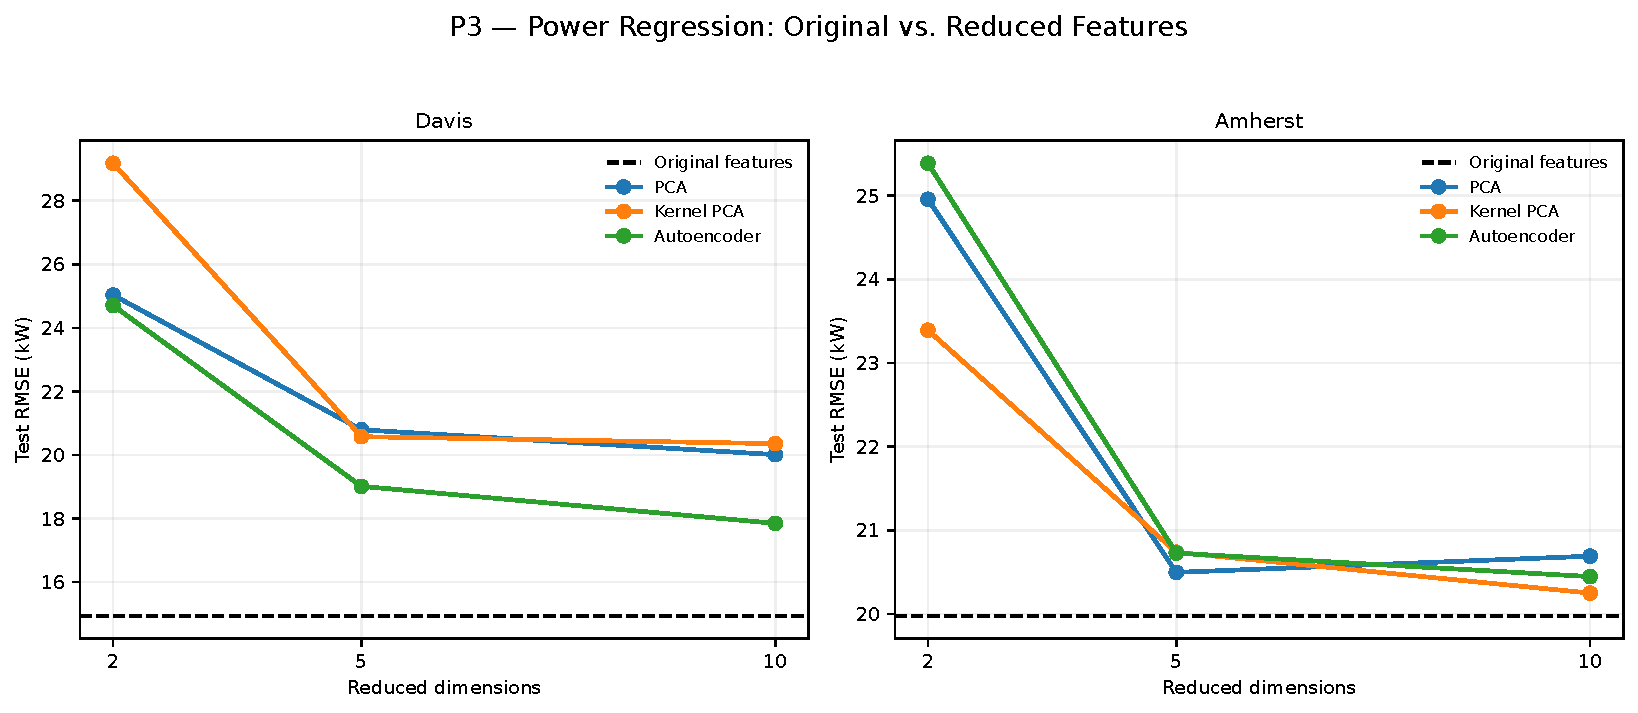
\includegraphics[width=\linewidth,height=5.53cm,keepaspectratio]{Figures/P3/P3_Regression_All_Methods.pdf}
\end{column}
\begin{column}{0.30\textwidth}
\factbox{Davis, $d=10$}{Autoencoder + SVR: 17.85\,kW vs 14.93\,kW raw.}\vspace{0.15cm}
\factbox{Amherst, $d=10$}{Kernel PCA + MLP: 20.25\,kW vs 19.97\,kW raw.}
\end{column}
\end{columns}
\footeridea{No reduced configuration beat the best full-feature model.}
\note{Regression shows the same pattern. In Davis the best compressed model, an autoencoder with
SVR, is about 3 kilowatts worse than raw features; in Amherst the gap is only 0.3 kilowatts.}
\end{frame}

\begin{frame}{P3 — Downstream models: PV power regression}
\sectiontag{P3 \quad RESULTS — 10-DIMENSIONAL INPUTS}
\smallmuted{RMSE (kW), lower is better; mean over three seeds.}\vspace{0.18cm}
\begin{columns}[T,onlytextwidth]
\begin{column}{0.486\textwidth}
\textbf{Davis}\hfill{\scriptsize raw best: 14.93}\par\vspace{0.12cm}
{\fontsize{8.8}{10.4}\selectfont
\setlength{\tabcolsep}{3.9pt}
\renewcommand{\arraystretch}{1.39}
\begin{tabular}{@{}lrrr@{}}\toprule
\textbf{Model} & \textbf{PCA} & \textbf{KPCA} & \textbf{AE}\\\midrule
Ridge & 24.09 & 26.63 & 22.44\\
RBF SVR & 27.98 & 24.32 & \textcolor{teal}{\textbf{17.85}}\\
RF & 20.09 & 20.68 & 20.35\\
XGBoost & 21.09 & 20.54 & 21.24\\
MLP & 20.01 & 20.36 & 17.86\\
\bottomrule\end{tabular}}
\end{column}
\begin{column}{0.486\textwidth}
\textbf{Amherst}\hfill{\scriptsize raw best: 19.97}\par\vspace{0.12cm}
{\fontsize{8.8}{10.4}\selectfont
\setlength{\tabcolsep}{3.9pt}
\renewcommand{\arraystretch}{1.39}
\begin{tabular}{@{}lrrr@{}}\toprule
\textbf{Model} & \textbf{PCA} & \textbf{KPCA} & \textbf{AE}\\\midrule
Ridge & 21.42 & 20.98 & 21.47\\
RBF SVR & 23.39 & 21.53 & 20.53\\
RF & 20.92 & 20.92 & 20.95\\
XGBoost & 20.90 & 20.91 & 20.75\\
MLP & 20.69 & \textcolor{teal}{\textbf{20.25}} & 20.45\\
\bottomrule\end{tabular}}
\end{column}
\end{columns}
\vspace{0.30cm}
\begin{beamercolorbox}[wd=\linewidth,sep=0.14cm]{block body}
\footnotesize In Davis the non-linear autoencoder gives the best compressed regressors (SVR and MLP, $\approx$17.9\,kW).
\end{beamercolorbox}
\note{The detailed regression table: in Davis both the best and second-best compressed regressors use
autoencoder features, so a non-linear bottleneck keeps more of the power-relevant information.}
\end{frame}

\begin{frame}{P4 — Preprocessing and label budgets}
\sectiontag{P4 \quad PREPROCESSING}
\begin{enumerate}\setlength\itemsep{0.43em}
\item Split chronologically into training and held-out test observations.
\item Inside the \textbf{training partition}, hide labels from 90\%, 70\% or 50\% of examples (seeded).
\item Train the supervised baseline and every SSL method on the \textbf{identical labeled subset}.
\item Only training inputs are pseudo-labeled or used for representation learning; never the test set.
\item Evaluate every method on the same \textbf{full held-out test set}.
\end{enumerate}
\footeridea{A gain is meaningful only against the supervised model with the same budget.}
\note{Labels are hidden only inside the training partition, with the seed controlling which ones.
The supervised baseline and the SSL methods see exactly the same labeled samples, so any difference
comes from the unlabeled data.}
\end{frame}

\begin{frame}{P4 — Macro-F1 and label-efficiency AUC}
\sectiontag{P4 \quad RESULTS — ACROSS BUDGETS}
\begin{columns}[T,totalwidth=\textwidth]
\begin{column}{0.59\textwidth}
\centering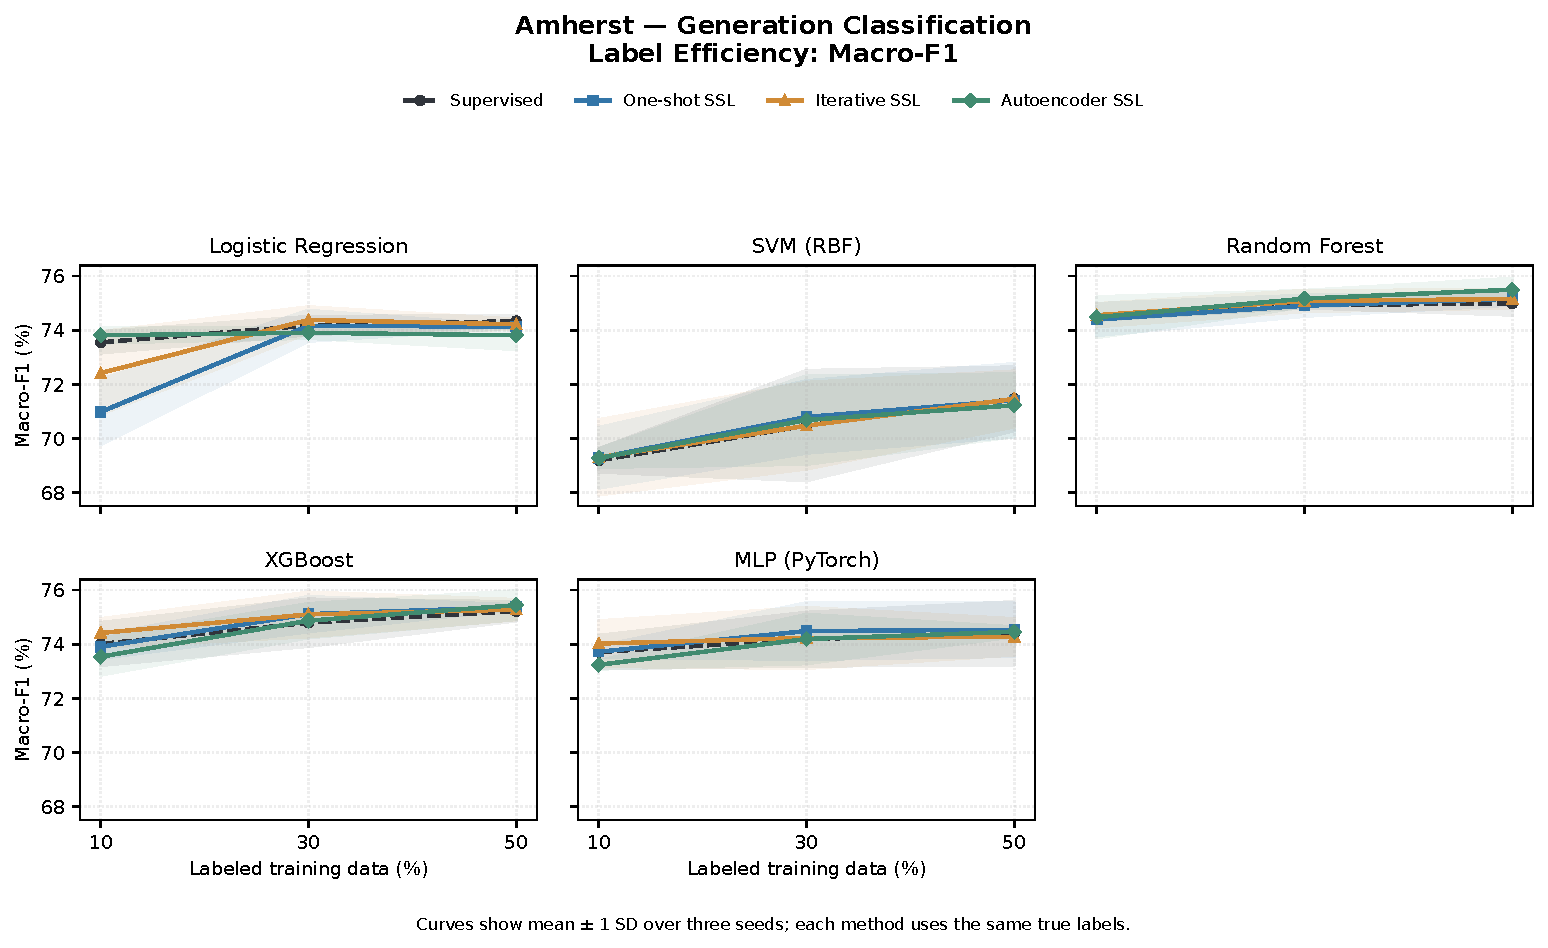
\includegraphics[width=\linewidth,height=4.99cm,keepaspectratio]{Figures/P4/P4_Amherst_Generation_Macro_F1_All_Models.pdf}
\smallmuted{Amherst Generation: macro-F1 vs 10/30/50\% labels}
\end{column}
\begin{column}{0.39\textwidth}
\textbf{XGBoost: normalized BA AUC}\par\vspace{0.10cm}
{\scriptsize\begin{tabular}{@{}lr@{}}\toprule
\textbf{Method} & \textbf{Mean $\pm$ SD}\\\midrule
Supervised & 0.747 $\pm$ 0.004 \\
One-shot SSL & 0.749 $\pm$ 0.001 \\
Iterative SSL & 0.749 $\pm$ 0.003 \\
Autoencoder SSL & 0.748 $\pm$ 0.006 \\
\bottomrule\end{tabular}}
\par\vspace{0.14cm}
\smallmuted{Area under the 10--50\% curve (Amherst generation); all differences are within one SD.}
\end{column}
\end{columns}
\footeridea{AUC summarizes the whole curve in one number; here it confirms ``no reliable SSL advantage''.}
\note{The assignment also asks for macro-F1 curves and an AUC summary. For XGBoost on Amherst
generation, all four strategies have essentially the same area under the curve.}
\end{frame}

\begin{frame}{P4 — Analysis: why are SSL gains so small?}
\sectiontag{P4 \quad ANALYSIS}
\begin{columns}[T,totalwidth=\textwidth]
\begin{column}{0.60\textwidth}
\centering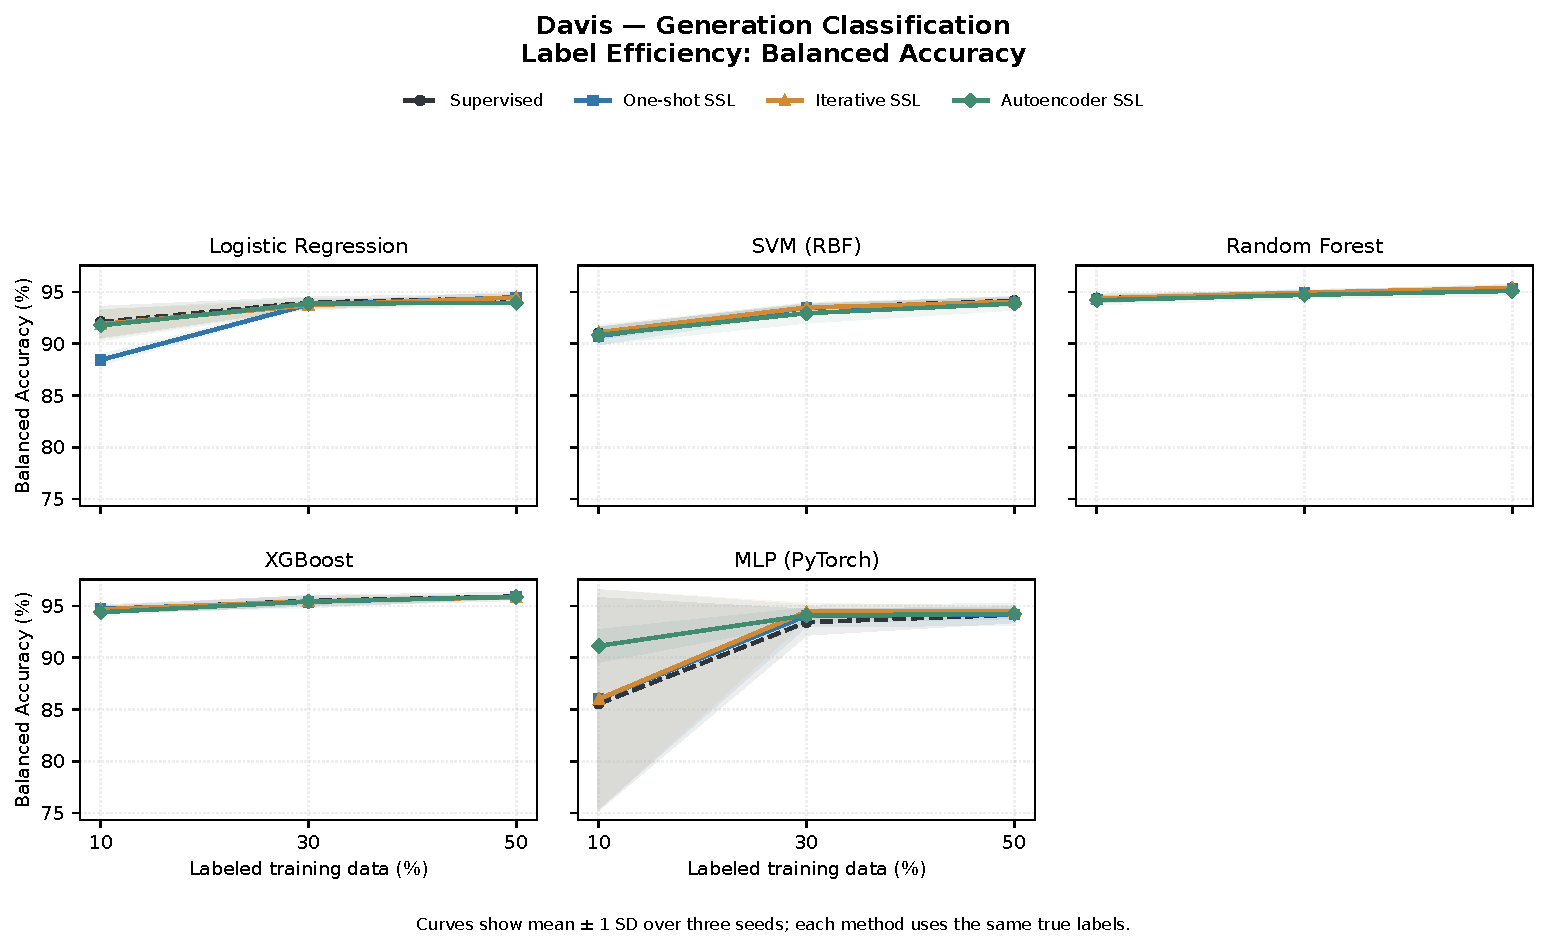
\includegraphics[width=\linewidth,height=5.3cm,keepaspectratio]{Figures/P4/P4_Davis_Generation_Balanced_Accuracy_All_Models.pdf}
\end{column}
\begin{column}{0.37\textwidth}
\factbox{1. Baselines near ceiling}{10\% of a multi-year sheet is still on the order of a thousand labels.}\vspace{0.1cm}
\factbox{2. Confirmation bias}{Pseudo-labels recycle errors: one-shot drops logistic regression 4 points on Amherst generation.}\vspace{0.1cm}
\factbox{3. Variance reduction}{MLP SD 10.2 $\to$ 1.5 with AE features.}
\end{column}
\end{columns}
\footeridea{SSL helps most as a stabilizer for data-hungry neural models at the smallest budgets.}
\note{Why so small? First, ten percent of a multi-year sheet is still around a thousand labels,
so strong models are already near their ceiling. Second, pseudo-labeling recycles the model's own
errors; for logistic regression on Amherst it actually costs four points. Third, where SSL does help
is variance: autoencoder features cut the MLP's seed spread from ten points to one and a half.}
\end{frame}

\begin{frame}{P5 — Preprocessing and fair comparison}
\sectiontag{P5 \quad PREPROCESSING}
\begin{enumerate}\setlength\itemsep{0.43em}
\item Davis training observations form the source; Amherst keeps a separate \textbf{chronological test set}.
\item Source-side transformations are fitted on Davis training data.
\item Only $k=10,\,50,\,100$ \textbf{labeled Amherst training samples} (seeded) are used for few-shot training or adaptation.
\item Amherst test labels are never used for training, calibration or fine-tuning.
\item All methods are scored on the \textbf{same Amherst test set}.
\end{enumerate}
\footeridea{Transfer gain = target-only RMSE $-$ transfer RMSE at the same $k$ and base model.}
\note{The comparison is kept fair: every method sees the same k Amherst labels, and the Amherst
test set is used only for scoring. Transfer gain is the target-only error minus the transfer error,
so a positive number means the source helped.}
\end{frame}

\begin{frame}{P5 — Classical transfer: what do the names mean?}
\sectiontag{P5 \quad MODELS EXPLAINED}
\begin{block}{1. Affine calibration — correct the source predictions}
\small Keep the Davis model; use the $k$ Amherst labels to fit a \textbf{scale} $a$ and \textbf{offset} $b$:
\[
\hat y_{\mathrm{Amherst}} = a\,\hat y_{\mathrm{Davis\ model}}(x) + b.
\]
Directly targets the scale bias found in P2.
\end{block}
\vspace{0.12cm}
\begin{block}{2. Joint calibrated pooling — use both cities}
\small Rescale the Davis targets to Amherst's output level, then fit one model on \textbf{calibrated Davis data + the $k$ Amherst samples}. Borrows Davis's many weather situations, respects Amherst's scale.
\end{block}
\note{Affine calibration keeps the Davis model and learns just two numbers, a scale and an offset,
from the Amherst labels. That directly attacks the scale problem from P2. Joint pooling goes
further: it rescales the Davis training targets to Amherst's level and trains one model on both
cities together.}
\end{frame}

\begin{frame}{P5 — Neural transfer: reuse a pretrained network}
\sectiontag{P5 \quad MODELS EXPLAINED}
\begin{block}{3. Frozen encoder + Ridge — reuse features, learn a small head}
\small Train an MLP on Davis, keep its hidden layers \textbf{frozen} as a feature extractor, and fit a new \textbf{Ridge} output layer on the $k$ Amherst labels.
\end{block}
\vspace{0.14cm}
\begin{block}{4. Partial fine-tuning — update only part of the network}
\small Start from the Davis-pretrained MLP, keep early layers fixed and \textbf{update the later layers} on Amherst labels.
\end{block}
\vspace{0.15cm}
\begin{beamercolorbox}[sep=0.13cm,wd=\linewidth]{block body}
\small \textbf{Why not retrain everything?} With 10--100 labels, limiting what is learned reduces overfitting and instability.
\end{beamercolorbox}
\note{The neural methods reuse the Davis network. The frozen-encoder method keeps the hidden layers
as fixed features and learns only a Ridge head. Partial fine-tuning updates only the last layers.
With so few labels, learning less is safer.}
\end{frame}

\begin{frame}{P5 — Results: RMSE vs number of target labels}
\sectiontag{P5 \quad RESULTS}
\begin{columns}[T,totalwidth=\textwidth]
\begin{column}{0.65\textwidth}
\centering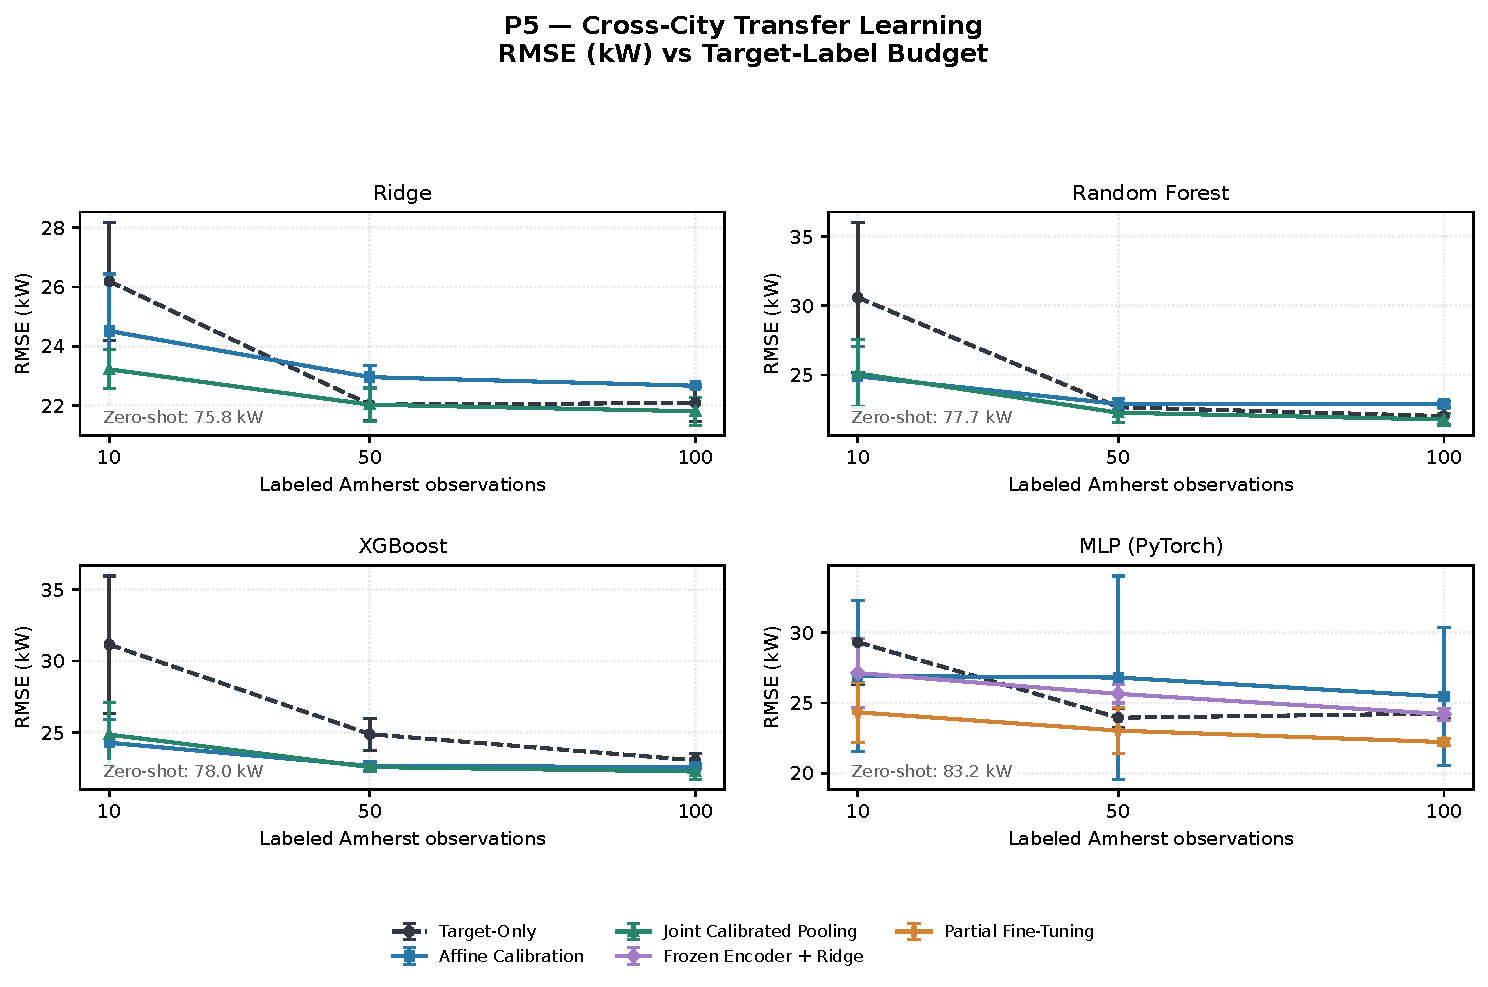
\includegraphics[width=\linewidth,height=5.55cm,keepaspectratio]{Figures/P5/P5_RMSE_Label_Efficiency_All_Models.pdf}
\end{column}
\begin{column}{0.32\textwidth}
\factbox{Source-only zero-shot}{Best Davis$\to$Amherst RMSE: \textbf{75.82\,kW} (Ridge), 59.6\% nRMSE.}\vspace{0.16cm}
\factbox{With 10 target labels}{Ridge target-only: 26.19\,kW\\Joint pooling: \textbf{23.22\,kW}.}
\end{column}
\end{columns}
\footeridea{Ten labels change the outcome dramatically; the source still adds on top of them.}
\note{Here is RMSE against the number of Amherst labels for each base model. Zero-shot is
annotated in each panel at around 76 to 83 kilowatts, far off the chart. With just ten labels,
every method is between about 23 and 31 kilowatts.}
\end{frame}

\begin{frame}{P5 — All strategies (held-out Amherst RMSE, kW)}
\sectiontag{P5 \quad RESULTS — FULL TABLE}
{\scriptsize
\setlength{\tabcolsep}{5pt}
\renewcommand{\arraystretch}{1.12}
\begin{tabular}{@{}llrrr@{}}\toprule
\textbf{Base model} & \textbf{Strategy} & \textbf{$k=10$} & \textbf{$k=50$} & \textbf{$k=100$}\\\midrule
Ridge & Target-only & 26.19 $\pm$ 1.99 & \cellcolor{softteal}\textbf{22.03 $\pm$ 0.53} & 22.09 $\pm$ 0.63\\
Ridge & Affine calibration & 24.52 $\pm$ 1.92 & 22.96 $\pm$ 0.39 & 22.67 $\pm$ 0.05\\
Ridge & Joint pooling & \cellcolor{softteal}\textbf{23.22 $\pm$ 0.66} & \cellcolor{softteal}\textbf{22.03 $\pm$ 0.58} & 21.81 $\pm$ 0.47\\
Random forest & Target-only & 30.60 $\pm$ 5.42 & 22.69 $\pm$ 0.37 & 22.04 $\pm$ 0.62\\
Random forest & Affine calibration & 24.92 $\pm$ 2.17 & 22.92 $\pm$ 0.42 & 22.91 $\pm$ 0.15\\
Random forest & Joint pooling & 25.12 $\pm$ 2.44 & 22.29 $\pm$ 0.71 & \cellcolor{softteal}\textbf{21.80 $\pm$ 0.42}\\
XGBoost & Target-only & 31.15 $\pm$ 4.79 & 24.90 $\pm$ 1.12 & 23.07 $\pm$ 0.46\\
XGBoost & Affine calibration & 24.30 $\pm$ 1.62 & 22.68 $\pm$ 0.32 & 22.60 $\pm$ 0.09\\
XGBoost & Joint pooling & 24.87 $\pm$ 2.26 & 22.60 $\pm$ 0.30 & 22.29 $\pm$ 0.53\\
MLP & Target-only & 29.31 $\pm$ 2.97 & 23.94 $\pm$ 0.67 & 24.24 $\pm$ 0.35\\
MLP & Affine calibration & 26.91 $\pm$ 5.39 & 26.80 $\pm$ 7.22 & 25.44 $\pm$ 4.92\\
MLP & Frozen encoder + Ridge & 27.12 $\pm$ 2.44 & 25.64 $\pm$ 0.65 & 24.20 $\pm$ 0.42\\
MLP & Partial fine-tuning & 24.33 $\pm$ 2.13 & 23.03 $\pm$ 1.63 & 22.21 $\pm$ 0.23\\
\bottomrule\end{tabular}}
\par\vspace{0.1cm}\smallmuted{Mean $\pm$ SD over three seeds; shaded = best at each budget.}
\note{This is the full table of every base model and strategy. Joint pooling is best at ten and
one hundred labels, and ties the Ridge target-only model at fifty.}
\end{frame}

\begin{frame}{P5 — Matched gain per base model}
\sectiontag{P5 \quad ANALYSIS — POSITIVE AND NEGATIVE TRANSFER}
{\footnotesize
\setlength{\tabcolsep}{6pt}
\renewcommand{\arraystretch}{1.22}
\begin{tabular}{@{}llrrr@{}}\toprule
\textbf{Base model} & \textbf{Strategy} & \textbf{$k=10$} & \textbf{$k=50$} & \textbf{$k=100$}\\\midrule
Ridge & Affine / Pooling & $+1.67$ / $+2.97$ & \textcolor{warn}{$-0.93$} / $+0.00$ & \textcolor{warn}{$-0.58$} / $+0.28$\\
Random forest & Affine / Pooling & $+5.68$ / $+5.48$ & \textcolor{warn}{$-0.23$} / $+0.40$ & \textcolor{warn}{$-0.87$} / $+0.24$\\
XGBoost & Affine / Pooling & $\mathbf{+6.85}$ / $+6.28$ & $+2.22$ / $+2.30$ & $+0.47$ / $+0.78$\\
MLP & Affine & $+2.40$ & \textcolor{warn}{$-2.86$} & \textcolor{warn}{$-1.20$}\\
MLP & Frozen enc. / Fine-tune & $+2.19$ / $+4.98$ & \textcolor{warn}{$-1.70$} / $+0.91$ & $+0.04$ / $+2.03$\\
\bottomrule\end{tabular}}
\vspace{0.2cm}
\begin{columns}[T,totalwidth=\textwidth]
\begin{column}{0.49\textwidth}
\factbox{Robust}{Joint pooling and partial fine-tuning are \emph{never} negative.}
\end{column}
\begin{column}{0.49\textwidth}
\factbox{Negative transfer}{Affine calibration hurts 3 of 4 models once $k\ge50$ (shown in orange).}
\end{column}
\end{columns}
\note{Looking model by model: the weak, high-variance learners gain most at ten labels, up to
6.85 kilowatts for XGBoost. Joint pooling and partial fine-tuning never hurt. Affine calibration
does cause negative transfer once there are fifty or more labels: a single scale and offset can't
fix errors that vary across conditions, and a model with enough Amherst data no longer needs it.}
\end{frame}



\fi
\end{document}